\documentclass[
  man,
  floatsintext,
  longtable,
  nolmodern,
  notxfonts,
  notimes,
  colorlinks=true,linkcolor=blue,citecolor=blue,urlcolor=blue]{apa7}

\usepackage{amsmath}
\usepackage{amssymb}
\usepackage{setspace}



\RequirePackage{longtable}
\RequirePackage{threeparttablex}

\usepackage{framed}


\makeatletter
\renewcommand{\paragraph}{\@startsection{paragraph}{4}{\parindent}%
	{0\baselineskip \@plus 0.2ex \@minus 0.2ex}%
	{-.5em}%
	{\normalfont\normalsize\bfseries\typesectitle}}

\renewcommand{\subparagraph}[1]{\@startsection{subparagraph}{5}{0.5em}%
	{0\baselineskip \@plus 0.2ex \@minus 0.2ex}%
	{-\z@\relax}%
	{\normalfont\normalsize\bfseries\itshape\hspace{\parindent}{#1}\textit{\addperi}}{\relax}}
\makeatother




\usepackage{longtable, booktabs, multirow, multicol, colortbl, hhline, caption, array, float, xpatch}
\usepackage{subcaption}


\renewcommand\thesubfigure{\Alph{subfigure}}
\setcounter{topnumber}{2}
\setcounter{bottomnumber}{2}
\setcounter{totalnumber}{4}
\renewcommand{\topfraction}{0.85}
\renewcommand{\bottomfraction}{0.85}
\renewcommand{\textfraction}{0.15}
\renewcommand{\floatpagefraction}{0.7}

\usepackage{tcolorbox}
\tcbuselibrary{listings,theorems, breakable, skins}
\usepackage{fontawesome5}

\definecolor{quarto-callout-color}{HTML}{909090}
\definecolor{quarto-callout-note-color}{HTML}{0758E5}
\definecolor{quarto-callout-important-color}{HTML}{CC1914}
\definecolor{quarto-callout-warning-color}{HTML}{EB9113}
\definecolor{quarto-callout-tip-color}{HTML}{00A047}
\definecolor{quarto-callout-caution-color}{HTML}{FC5300}
\definecolor{quarto-callout-color-frame}{HTML}{ACACAC}
\definecolor{quarto-callout-note-color-frame}{HTML}{4582EC}
\definecolor{quarto-callout-important-color-frame}{HTML}{D9534F}
\definecolor{quarto-callout-warning-color-frame}{HTML}{F0AD4E}
\definecolor{quarto-callout-tip-color-frame}{HTML}{02B875}
\definecolor{quarto-callout-caution-color-frame}{HTML}{FD7E14}

%\newlength\Oldarrayrulewidth
%\newlength\Oldtabcolsep


\usepackage{hyperref}
\usepackage[protrusion=true]{microtype}



\providecommand{\tightlist}{%
  \setlength{\itemsep}{0pt}\setlength{\parskip}{0pt}}
\usepackage{longtable,booktabs,array}
\newcounter{none} % for unnumbered tables
\usepackage{calc} % for calculating minipage widths
% Correct order of tables after \paragraph or \subparagraph
\usepackage{etoolbox}
\makeatletter
\patchcmd\longtable{\par}{\if@noskipsec\mbox{}\fi\par}{}{}
\makeatother
% Allow footnotes in longtable head/foot
\IfFileExists{footnotehyper.sty}{\usepackage{footnotehyper}}{\usepackage{footnote}}
\makesavenoteenv{longtable}

\usepackage{graphicx}
\makeatletter
\newsavebox\pandoc@box
\newcommand*\pandocbounded[1]{% scales image to fit in text height/width
  \sbox\pandoc@box{#1}%
  \Gscale@div\@tempa{\textheight}{\dimexpr\ht\pandoc@box+\dp\pandoc@box\relax}%
  \Gscale@div\@tempb{\linewidth}{\wd\pandoc@box}%
  \ifdim\@tempb\p@<\@tempa\p@\let\@tempa\@tempb\fi% select the smaller of both
  \ifdim\@tempa\p@<\p@\scalebox{\@tempa}{\usebox\pandoc@box}%
  \else\usebox{\pandoc@box}%
  \fi%
}
% Set default figure placement to htbp
\def\fps@figure{htbp}
\makeatother


% definitions for citeproc citations
\NewDocumentCommand\citeproctext{}{}
\NewDocumentCommand\citeproc{mm}{%
  \begingroup\def\citeproctext{#2}\cite{#1}\endgroup}
\makeatletter
 % allow citations to break across lines
 \let\@cite@ofmt\@firstofone
 % avoid brackets around text for \cite:
 \def\@biblabel#1{}
 \def\@cite#1#2{{#1\if@tempswa , #2\fi}}
\makeatother
\newlength{\cslhangindent}
\setlength{\cslhangindent}{1.5em}
\newlength{\csllabelwidth}
\setlength{\csllabelwidth}{3em}
\newenvironment{CSLReferences}[2] % #1 hanging-indent, #2 entry-spacing
 {\begin{list}{}{%
  \setlength{\itemindent}{0pt}
  \setlength{\leftmargin}{0pt}
  \setlength{\parsep}{0pt}
  % turn on hanging indent if param 1 is 1
  \ifodd #1
   \setlength{\leftmargin}{\cslhangindent}
   \setlength{\itemindent}{-1\cslhangindent}
  \fi
  % set entry spacing
  \setlength{\itemsep}{#2\baselineskip}}}
 {\end{list}}
\usepackage{calc}
\newcommand{\CSLBlock}[1]{\hfill\break\parbox[t]{\linewidth}{\strut\ignorespaces#1\strut}}
\newcommand{\CSLLeftMargin}[1]{\parbox[t]{\csllabelwidth}{\strut#1\strut}}
\newcommand{\CSLRightInline}[1]{\parbox[t]{\linewidth - \csllabelwidth}{\strut#1\strut}}
\newcommand{\CSLIndent}[1]{\hspace{\cslhangindent}#1}





\usepackage{newtx}

\defaultfontfeatures{Scale=MatchLowercase}
\defaultfontfeatures[\rmfamily]{Ligatures=TeX,Scale=1}





\title{Illusory Traits as the Number of Timepoints Increases: a New
Method to Account for Unobserved Time-Varying Confounding}


\shorttitle{Illusory Traits as the Number of Timepoints Increases}


\usepackage{etoolbox}








\authorsnames{Axel Zweistra (7663200),Jeroen Mulder,Ellen Hamaker}





\affiliation{
{Department of Methods and Statistics, Faculty of Social and Behavioural
Sciences, Utrecht University}}




\leftheader{(7663200), Mulder and Hamaker}



\abstract{The cross-lagged panel model (CLPM) is a popular option for
researchers in the social sciences interested in multivariate
longitudinal data. Often criticized as being too restrictive in
assumptions concerning confounding, this paper presents an extension of
the CLPM aimed at controlling for both time-varying and time-invariant
confounding. This development is heavily inspired by the `illusory
trait' finding, showing that the RI-CLPM can not only correct for the
time-invariant confounding it was designed to correct for, but also for
time-varying confounding. The performance of this new model, the
segmented random intercept cross-lagged panel model (SRI-CLPM) is
examined in a series of Monte Carlo simulations. These show the model
outperforming the RI-CLPM and CLPM in retrieving less biased estimates
of cross-lagged parameters, at a slight increase in standard errors.
This effect becomes more pronounced as more timepoints are considered,
as the RI-CLPM starts to be unable to correct for time-varying
confounding. A possible further extension of the SRI-CLPM is also
explored, aimed at separating the variance associated with time-varying
and time-invariant confounding. }

\keywords{CLPM, RI-CLPM, Cross-Lagged Panel Modeling, Illusory
Traits, SRI-CLPM, Time-Varying Confounding}

\authornote{\par{\addORCIDlink{Axel Zweistra
(7663200)}{0009-0000-8790-4608}}\par{\addORCIDlink{Jeroen
Mulder}{0000-0002-5553-0856}} 

\par{   The author(s) declare that there were no conflicts of interest
with respect to the authorship or the publication of this article.
Thesis for the Research Master Methodology and Statistics for the
Behavioural, Biomedical and Social Sciences. Candidate journal is
Structural Equation Modeling. FETC Registration Number 25-2051.
Generative AI was used for the generation of code, all code was reviewed
and edited manually with the first author taking full responsibility for
the final analysis. Code repository can be found at
https://github.com/AxelZweistra/Thesis-Illusionary-Traits    }
\par{Correspondence concerning this article should be addressed to Axel
Zweistra (7663200), Department of Methods and Statistics, Faculty of
Social and Behavioural Sciences, Utrecht University, Padualaan
14, Utrecht 3584 CH, The
Netherlands, Email: \href{mailto:a.p.zweistra@uu.nl}{a.p.zweistra@uu.nl}}
}

\makeatletter
\let\endoldlt\endlongtable
\def\endlongtable{
\hline
\endoldlt
}
\makeatother

\urlstyle{same}



\usepackage{booktabs}
\usepackage{longtable}
\usepackage{array}
\usepackage{multirow}
\usepackage{wrapfig}
\usepackage{float}
\usepackage{colortbl}
\usepackage{pdflscape}
\usepackage{tabu}
\usepackage{threeparttable}
\usepackage{threeparttablex}
\usepackage[normalem]{ulem}
\usepackage{makecell}
\usepackage{xcolor}
\AtBeginDocument{\thispagestyle{empty}}
\makeatletter
\@ifpackageloaded{caption}{}{\usepackage{caption}}
\AtBeginDocument{%
\ifdefined\contentsname
  \renewcommand*\contentsname{Table of contents}
\else
  \newcommand\contentsname{Table of contents}
\fi
\ifdefined\listfigurename
  \renewcommand*\listfigurename{List of Figures}
\else
  \newcommand\listfigurename{List of Figures}
\fi
\ifdefined\listtablename
  \renewcommand*\listtablename{List of Tables}
\else
  \newcommand\listtablename{List of Tables}
\fi
\ifdefined\figurename
  \renewcommand*\figurename{Figure}
\else
  \newcommand\figurename{Figure}
\fi
\ifdefined\tablename
  \renewcommand*\tablename{Table}
\else
  \newcommand\tablename{Table}
\fi
}
\@ifpackageloaded{float}{}{\usepackage{float}}
\floatstyle{ruled}
\@ifundefined{c@chapter}{\newfloat{codelisting}{h}{lop}}{\newfloat{codelisting}{h}{lop}[chapter]}
\floatname{codelisting}{Listing}
\newcommand*\listoflistings{\listof{codelisting}{List of Listings}}
\makeatother
\makeatletter
\makeatother
\makeatletter
\@ifpackageloaded{caption}{}{\usepackage{caption}}
\@ifpackageloaded{subcaption}{}{\usepackage{subcaption}}
\makeatother

% From https://tex.stackexchange.com/a/645996/211326
%%% apa7 doesn't want to add appendix section titles in the toc
%%% let's make it do it
\makeatletter
\xpatchcmd{\appendix}
  {\par}
  {\addcontentsline{toc}{section}{\@currentlabelname}\par}
  {}{}
\makeatother

%% Disable longtable counter
%% https://tex.stackexchange.com/a/248395/211326

\usepackage{etoolbox}

\makeatletter
\patchcmd{\LT@caption}
  {\bgroup}
  {\bgroup\global\LTpatch@captiontrue}
  {}{}
\patchcmd{\longtable}
  {\par}
  {\par\global\LTpatch@captionfalse}
  {}{}
\apptocmd{\endlongtable}
  {\ifLTpatch@caption\else\addtocounter{table}{-1}\fi}
  {}{}
\newif\ifLTpatch@caption
\makeatother

\begin{document}

\maketitle




\setlength\LTleft{0pt}



\ifdefined\Shaded\renewenvironment{Shaded}{\begin{snugshade}\begin{singlespace}}{\end{singlespace}\end{snugshade}}\fi

\setlength{\cslhangindent}{0.5in}

When researchers are concerned with studying how two variables interact
over time, a helpful technique is the estimation of cross-lagged
parameters (\citeproc{ref-orthTestingProspectiveEffects2021}{Orth,
Clark, Donnellan, \& Robins, 2021}) . Cross-lagged parameters predict
the change in an outcome variable based on a previous measurement of the
other variable, while controlling for the score on the outcome variable
at the preceding occasion through an autoregressive parameter. Models
that include these parameters, such as the cross-lagged panel model
(CLPM, \citeproc{ref-duncanLinearModelsTwowave1969}{Duncan, 1969}), are
widely used in the social sciences. A major concern when using these
estimates for causal inference purposes is the possibility of them being
affected by unobserved confounding
(\citeproc{ref-hamakerCritiqueCrosslaggedPanel2015}{Hamaker, Kuiper, \&
Grasman, 2015};
\citeproc{ref-rogosaCritiqueCrosslaggedCorrelation1980}{Rogosa, 1980}).

Confounding refers to the process by which the relationship between two
variables is at least partially explained through the causal effects a
third variable has on them both. In longitudinal research, we can
broadly classify confounding into two types: time-varying and
time-invariant. The CLPM has been criticized as having its cross-lagged
parameter estimation confounded by stable, trait-like between-person
differences (\citeproc{ref-hamakerCritiqueCrosslaggedPanel2015}{Hamaker
et al., 2015}; \citeproc{ref-lucasWhyCrossLaggedPanel2023}{Lucas,
2023}). Models have therefore been developed that aim to control for
these time-invariant confounders, such as the random-intercept
cross-lagged panel model (RI-CLPM,
\citeproc{ref-hamakerCritiqueCrosslaggedPanel2015}{Hamaker et al.,
2015}) and alternatives such as the Trait-State-Error model
(\citeproc{ref-kennyTraitstateerrorModelMultiwave1995}{Kenny \& Zautra,
1995}). These models are designed to take away the influence of
time-invariant confounding by modeling them through the inclusion of
latent variables. In the RI-CLPM this is achieved by specifying a random
intercept, that is, a latent variable with factor loadings constrained
to 1 on all instances of a variable. This essentially centers the
variables around the mean value of an individual case (assuming that
mean does not change over time), a technique inspired by the multilevel
modeling literature. In doing so the model separates stable
between-person variation (e.g.~genetic predisposition, personality
traits) from within-person fluctuations. This is then argued to be a
better representation of the theoretical model, compared to the simpler
CLPM which assumes individual cases have the same underlying mean
(\citeproc{ref-lucasWhyCrossLaggedPanel2023}{Lucas, 2023}). These
models, and other related approaches, have been widely adopted by
researchers. An understudied topic however, is how to control for
unobserved time-varying confounding.

One approach in dealing with time-varying confounding, developed by
Kenny and McCoach (\citeproc{ref-kennyRulingOutLatent2025}{2025}), is
the Latent Time-Varying Confounder model (LTVC). This is a model that
aims to test the alternative hypothesis that all covariation between two
variables can be explained by a time-varying confounder. The authors
claim that a well-fitting LTVC only means that the possibility of all
covariation being explained by a time-varying confounder cannot be ruled
out (\citeproc{ref-kennyRulingOutLatent2025}{Kenny \& McCoach, 2025}).
While useful, this means it is not able to retrieve parameter estimates
for the model of theoretical interest while controlling for time-
varying confounding. The authors do show a model, the LTVC-CLPM, which
as the name suggests is a combination of both models, that aims to
remedy this limitation. They note however, that they were not able to
validate the model due to poor model fit and anomalous parameter
estimates. In this paper, we will take a different approach to modeling
time- varying confounding by considering systems of time-varying
confounding, rather than one underlying confounding variable.

A recent paper by Bailey et al.
(\citeproc{ref-baileyIllusoryTraitsWrong2024}{2024}) investigated the
performance of a bivariate RI- CLPM in the presence of systems of
time-varying confounding. They demonstrated that finding a significant
random intercept variance does not necessarily imply there was a time-
invariant confounder in the data generating process. Instead, when there
are many different time-varying confounders present, each having only a
small effect on each other and the variables of interest, fitting a
RI-CLPM without including the confounders estimates a significant random
intercept variance. Therefore the model seems to find evidence for the
existence of a stable, between person `trait'. Bailey et al.
(\citeproc{ref-baileyIllusoryTraitsWrong2024}{2024}) refer to this
phenomenon as `illusory traits', underlining these are not truly
underlying between person differences. Surprisingly, the addition of the
random intercept in the RI-CLPM controls for the presence of this
time-varying confounding, allowing the model to retrieve less biased
estimates of cross-lagged parameters than the CLPM. Therefore, Bailey
and colleagues caution researchers against interpreting significant
random intercept variance as evidence of a stable trait, yet still
advise researchers to choose a RI-CLPM over a CLPM. The question arising
is what happens to these illusory traits in the long run. Bailey and
colleagues (\citeproc{ref-baileyIllusoryTraitsWrong2024}{2024})
simulated datasets with only five timepoints. The authors show the
process behind estimating the illusory traits by plotting the rank order
stability with and without the time-varying confounding. The
autocorrelation between measurements decreases asymptotically to zero,
but this decay is slowed by the time-varying confounding. They do not
show however, how the performance of the RI-CLPM develops as more
timepoints are considered. Since the data were generated according to a
stationary process, meaning the underlying distributions of the
variables do not change over time
(\citeproc{ref-kirchgassnerIntroductionModernTime2008}{Kirchgässner \&
Wolters, 2008, pp. 12--12}), we expect any excess stability introduced
by the time-varying confounders to dissipate over time. In other words,
given enough time, the process will return to fluctuate around it's mean
value.

Investigating what happens when the number of timepoints increases is
especially relevant given the recent developments which allow for the
collection of more and more measurements through devices like
smartphones and smartwatches. This type of data is referred to as
intensive longitudinal data (ILD) and is characterized by many
measurements of variables densely packed in time
(\citeproc{ref-hoyleHANDBOOKSTRUCTURALEQUATION2023}{Hamaker, Asparouhov,
\& Muthén, 2023}). We can contrast this with panel data, which are
characterized by only a few measurements in study lengths measured in
weeks or months, rather than days. This density of measurements allows
researchers to study dynamics on small timespans, such as within a
single day
(\citeproc{ref-hamakerAnalysisIntensiveLongitudinal2025}{Hamaker,
2025}). However, this can be perceived as burdensome to participants,
given the frequency with which a participant is asked to answer a
psychological measure. It is therefore also doubtful whether this type
of data collection allows for the measurement of all potential
confounders of importance on every timepoint, due to the substantial
extra burden this poses to participants. Given the interest in these
studies and their increased feasibility, assessing the performance of
commonly used models with confounding in ILD is of substantial
importance. The aim of this paper is twofold. First, we aim to
investigate the expectation that the RI-CLPM is a less effective way of
dealing with time-varying unobserved confounders as the number of
timepoints increases, and that in the long-run its performance
approaches that of the CLPM. Second, we aim to design a model that can
control for time-varying confounding by introducing a model we refer to
as the Segmented Random Intercept Cross-Lagged Panel Model (SRI-CLPM).
This model aims to control for time-varying confounding by specifying
random intercepts for segments of the total timespan of the study,
inspired by the illusory trait finding. The rest of this paper is
structured as follows. We start by extending the simulation done by
Bailey et al. (\citeproc{ref-baileyIllusoryTraitsWrong2024}{2024}) to
scenarios with more timepoints to see whether the illusory traits indeed
largely disappear in the long run; we expect that this will go
hand-in-hand with an increase in bias in the cross-lagged parameters
which will approximate that of the CLPM as the number of timepoints
increases. Subsequently, we present the SRI-CLPM as a way to leverage
the finding of Bailey at el. in the context of increasing number of
timepoints, and perform an explorative study of an extension intended to
be able to separate time-invariant and time-varying confounding. We
simulate data and assess the performance of the SRI- CLPM under varying
segment timespans and covariance constraints. Lastly, we provide an
overall discussion and look ahead to possible future developments.

The aim of this paper is threefold. First, we will investigate whether
our expectation is correct that the RI-CLPM becomes a less effective way
of dealing with time-varying unobserved confounders as the number of
timepoints increases, and that in the long-run its performance
approaches that of the CLPM. Second, we will present a new model to
handle time-varying confounding as the number of timepoints increases:
the Segmented Random Intercept Cross-Lagged Panel Model (SRI-CLPM),
which controls for time-varying confounding through the inclusion of
random intercepts for segments of the total timespan of the study.
Third, we will present an extension of the SRI-CLPM with a global random
intercept (SGRI-CLPM), aimed at separating time-invariant from
time-varying confounding. The remainder of this paper is structured as
follows. We start by extending the simulation done by Bailey et al.
(\citeproc{ref-baileyIllusoryTraitsWrong2024}{2024}) to scenarios with
more timepoints to see whether the illusory traits indeed largely
disappear in the long run; we expect that this will go hand-in-hand with
an increase in bias in the cross-lagged parameters which will
approximate that of the CLPM as the number of timepoints increases.
Subsequently, we present the SRI-CLPM as a way to leverage the finding
of Bailey at el. in the context of an increasing number of timepoints,
and assess its ability to retrieve unbiased estimates of the
cross-lagged parameters under time-varying confounding. Thereafter, we
present the SGRI-CLPM and investigate whether it is possible to separate
confounding into a time-varying and time-invariant component using this
extension. Lastly, we provide an overall discussion and look ahead to
possible future developments.

\section{Illusory Traits in the RI-CLPM as the Number of Timepoints
Increases}\label{illusory-traits-in-the-ri-clpm-as-the-number-of-timepoints-increases}

We hypothesize that as the number of timepoints increases, the illusory
traits will disappear (that is, their variance will go to zero), and
that this development goes hand-in-hand with a deterioration of the
ability of the RI-CLPM to retrieve relatively unbiased cross-lagged
parameter estimates. We therefore build on the simulations done by
Bailey et al. (\citeproc{ref-baileyIllusoryTraitsWrong2024}{2024}) by
considering the effect of more timepoints. In addition, we also vary the
number of time-varying confounders and the strength of the
autoregressive effects across all variables to illustrate the role of
temporal stability in the observed processes.

\subsection{Extending the Simulation by Bailey and
colleagues}\label{extending-the-simulation-by-bailey-and-colleagues}

The data generating mechanism is adapted from the original illusory
trait paper by Bailey et al.
(\citeproc{ref-baileyIllusoryTraitsWrong2024}{2024}), largely following
their provided R-code. We use the same underlying parameter values they
specified as the defaults, only deviating from this to investigate
particular properties. We introduce their data generating mechanism
here, but refer to the original paper for a more in-depth discussion of
the parameter value choices. A schematic representation of the data
generating mechanism can be found in Figure~\ref{fig-DGM}. The data
generating mechanism consists of a bivariate CLPM with the addition of
systems of time-varying unobserved confounding. The relationships
between the observed variables \(X\) and \(Y\) are expressed in the
autoregressive effects and the cross-lagged effects.

In the first simulation, we generate data according to the data
generating mechanism, with conditions varying the number of unobserved
confounders on both variables and varying the autoregressive effects for
all variables (observed or unobserved). We will then attempt to
accurately retrieve estimates of the cross-lagged parameters under
confounding, fitting models only on the observed variables X and Y. We
vary the number of unobserved confounders on each variable to be either
4 or 6, resulting in a total number of 8 or 12 respectively. The system
(or grouping) of unobserved confounders on one variable has the same
parameter values with themselves and their observed variable as before;
cross-lagged effects of .1 and autoregressive effects varying to be .2
or .3. Additionally, the two systems weakly influence each other, with
all confounders on \(X\) having a lagged effect of .01 on the
confounders on \(Y\) and vice versa. Time-specific residual variances
were specified to be .5. After specifying the model, we sample from the
stationary covariance matrix of a single timepoint (see equation 2.1.39
in \citeproc{ref-lutkepohlNewIntroductionMultiple2007a}{Lütkepohl,
2007}) following the procedure in the original paper. This approach has
the benefit of not requiring to start up the process and wait for it to
reach its stationary state. We take a large sample of 20 thousand cases,
ensuring we can clearly estimate the degree of bias in the cross-lagged
parameters without the influence of sampling variation.

\begin{figure}[H]

\caption{\label{fig-DGM}Schematic representation of the data generating
mechanism adapted from Bailey et al.~Triple dots represent left out
intermediary variables for visual clarity.}

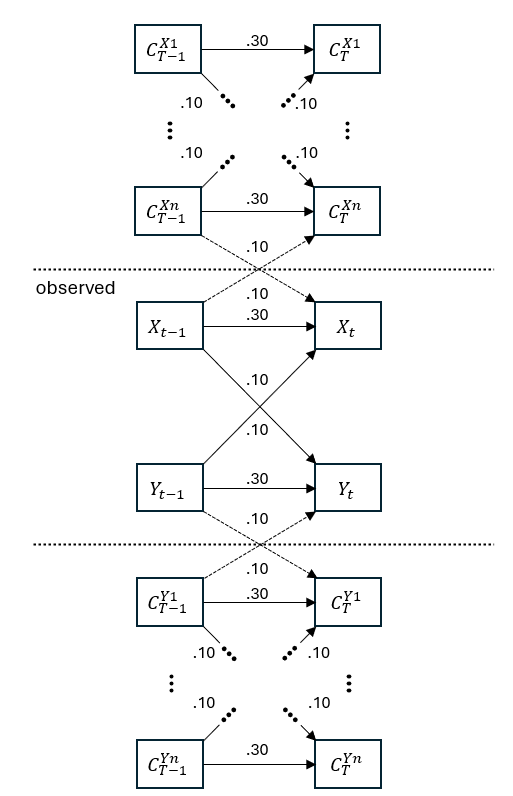
\includegraphics[width=0.45\linewidth,height=\textheight,keepaspectratio]{images/DGM.png}

\end{figure}%

\subsection{Stationarity \& Ergodicity}\label{stationarity-ergodicity}

As mentioned before, we simulate data from a stationary process, meaning
the properties of the underlying data distributions do not change over
time. Stationarity is often defined in terms of the first two moments,
which implies that the mean, variances and covariances of a process are
invariant over time; in this case, the process is said to be weakly
stationary
(\citeproc{ref-kirchgassnerIntroductionModernTime2008}{Kirchgässner \&
Wolters, 2008, pp. 22--13}). In the current context, the data that are
generated also conform to strict stationarity, meaning the third and
fourth moments also do not change over time. This is automatically the
case when generating data along a multivariate normal distribution,
since its third central moment is zero (the distribution is symmetric),
and its fourth central moment is a function of the covariances, which do
not change over time as follows from weak stationarity. To ensure the
data generating process is stationary, the autoregressive and
cross-lagged parameters have to fall within a particular range,
depending on their specific combination; if these requirements are not
met, the process would be non-stationarity and diverge (see Bailey et
al. (\citeproc{ref-baileyIllusoryTraitsWrong2024}{2024}) for an
example).

Since the data for each individual in the sample are generated according
to the same time series process with the exact same parameter values,
these data can be considered to reflect ergodicity. A process can be
said to be ergodic if the result of taking a pooled statistic aggregated
over time is equal to taking the pooled statistic aggregated over
multiple participants. For this to be the case two conditions need to
hold: the underlying data distributions do not change over time
(stationarity) and all participants need to be so similar as for each
participant to be replaceable with a randomly chosen other participant
in the sample (\citeproc{ref-hunterWhatErgodicityMeans2024}{Hunter,
Fisher, \& Geier, 2024}). This means that not only does every individual
case fluctuate around a time-invariant mean with a time-invariant
variance, but that every individual case fluctuates around the
\emph{same} mean. Additionally, in an ergodic process the same dynamics
hold for every individual case, and inferences made in the sample can be
generalized to individuals outside the sample
(\citeproc{ref-speelmanMostPsychologicalResearchers2024}{Speelman,
Parker, Rapley, \& McGann, 2024}). Especially important for our purposes
is that this means there are no long-run stable mean differences between
cases that could be estimated as an illusory trait.

After generating 75 occasions using the model described above, we first
select only the first three timepoints of the observed variables \(X\)
and \(Y\) and analyze them with the CLPM and RI-CLPM, as this is the
minimum number of timepoints for the latter model to be identified.
Subsequently, we select the first six timepoints and fit the two models
to these, and we continue this process in steps of three until we reach
models estimated on all 75 timepoints of \(X\) and \(Y\). These steps of
three are chosen to limit computational cost when estimating models of
this size. Parameters are constrained to be equal over time (e.g.~the
autoregression between \(X_{t1}\) and \(X_{t2}\) is equal to the
autoregression between \(X_{t2}\) and \(X_{t3}\)) corresponding to a
stationary process. All analyses are performed in R 4.3.1
(\citeproc{ref-R4.3.1}{R Core Team, 2023}) with models being estimated
using maximum likelihood as implemented in lavaan 0.6-17
(\citeproc{ref-rosseelLavaanPackageStructural2012}{Rosseel, 2012}).

\subsection{Results}\label{results}

Figure~\ref{fig-sim1_2x2} shows the bias in the cross-lagged parameter
from \(X\) to \(Y\), together with the estimated variance of the random
intercept~for \(X\), for each combination of the number of confounders
and autoregressive effects. We choose to display only one of the
cross-lagged parameters and one of the random intercepts since the model
is symmetrical, and as such the results are virtually identical for the
other parameters. As expected for all conditions, the illusory trait
variance decreases as the number of timepoints increases. The bias in
the cross-lagged parameter rises accordingly, illustrating the direct
relationship between the illusory trait variance and bias in
cross-lagged parameters. The data generating mechanism conditions show
that more confounders (right column versus left column), or a more
stable process due to higher autoregressive effects (bottom row versus
top row) are associated with a larger variance for the illusory trait,
and a slower decline of this variance as the number of timepoints
increases.

\begin{figure}[H]

\caption{\label{fig-sim1_2x2}Bias in the cross-lagged parameter and
random intercept variance per condition. α = autoregressive effects of
all variables (observed or unobserved), Confounders = number of
unobserved confounders on both observed variables. Highlighted panel has
different y-axis.}

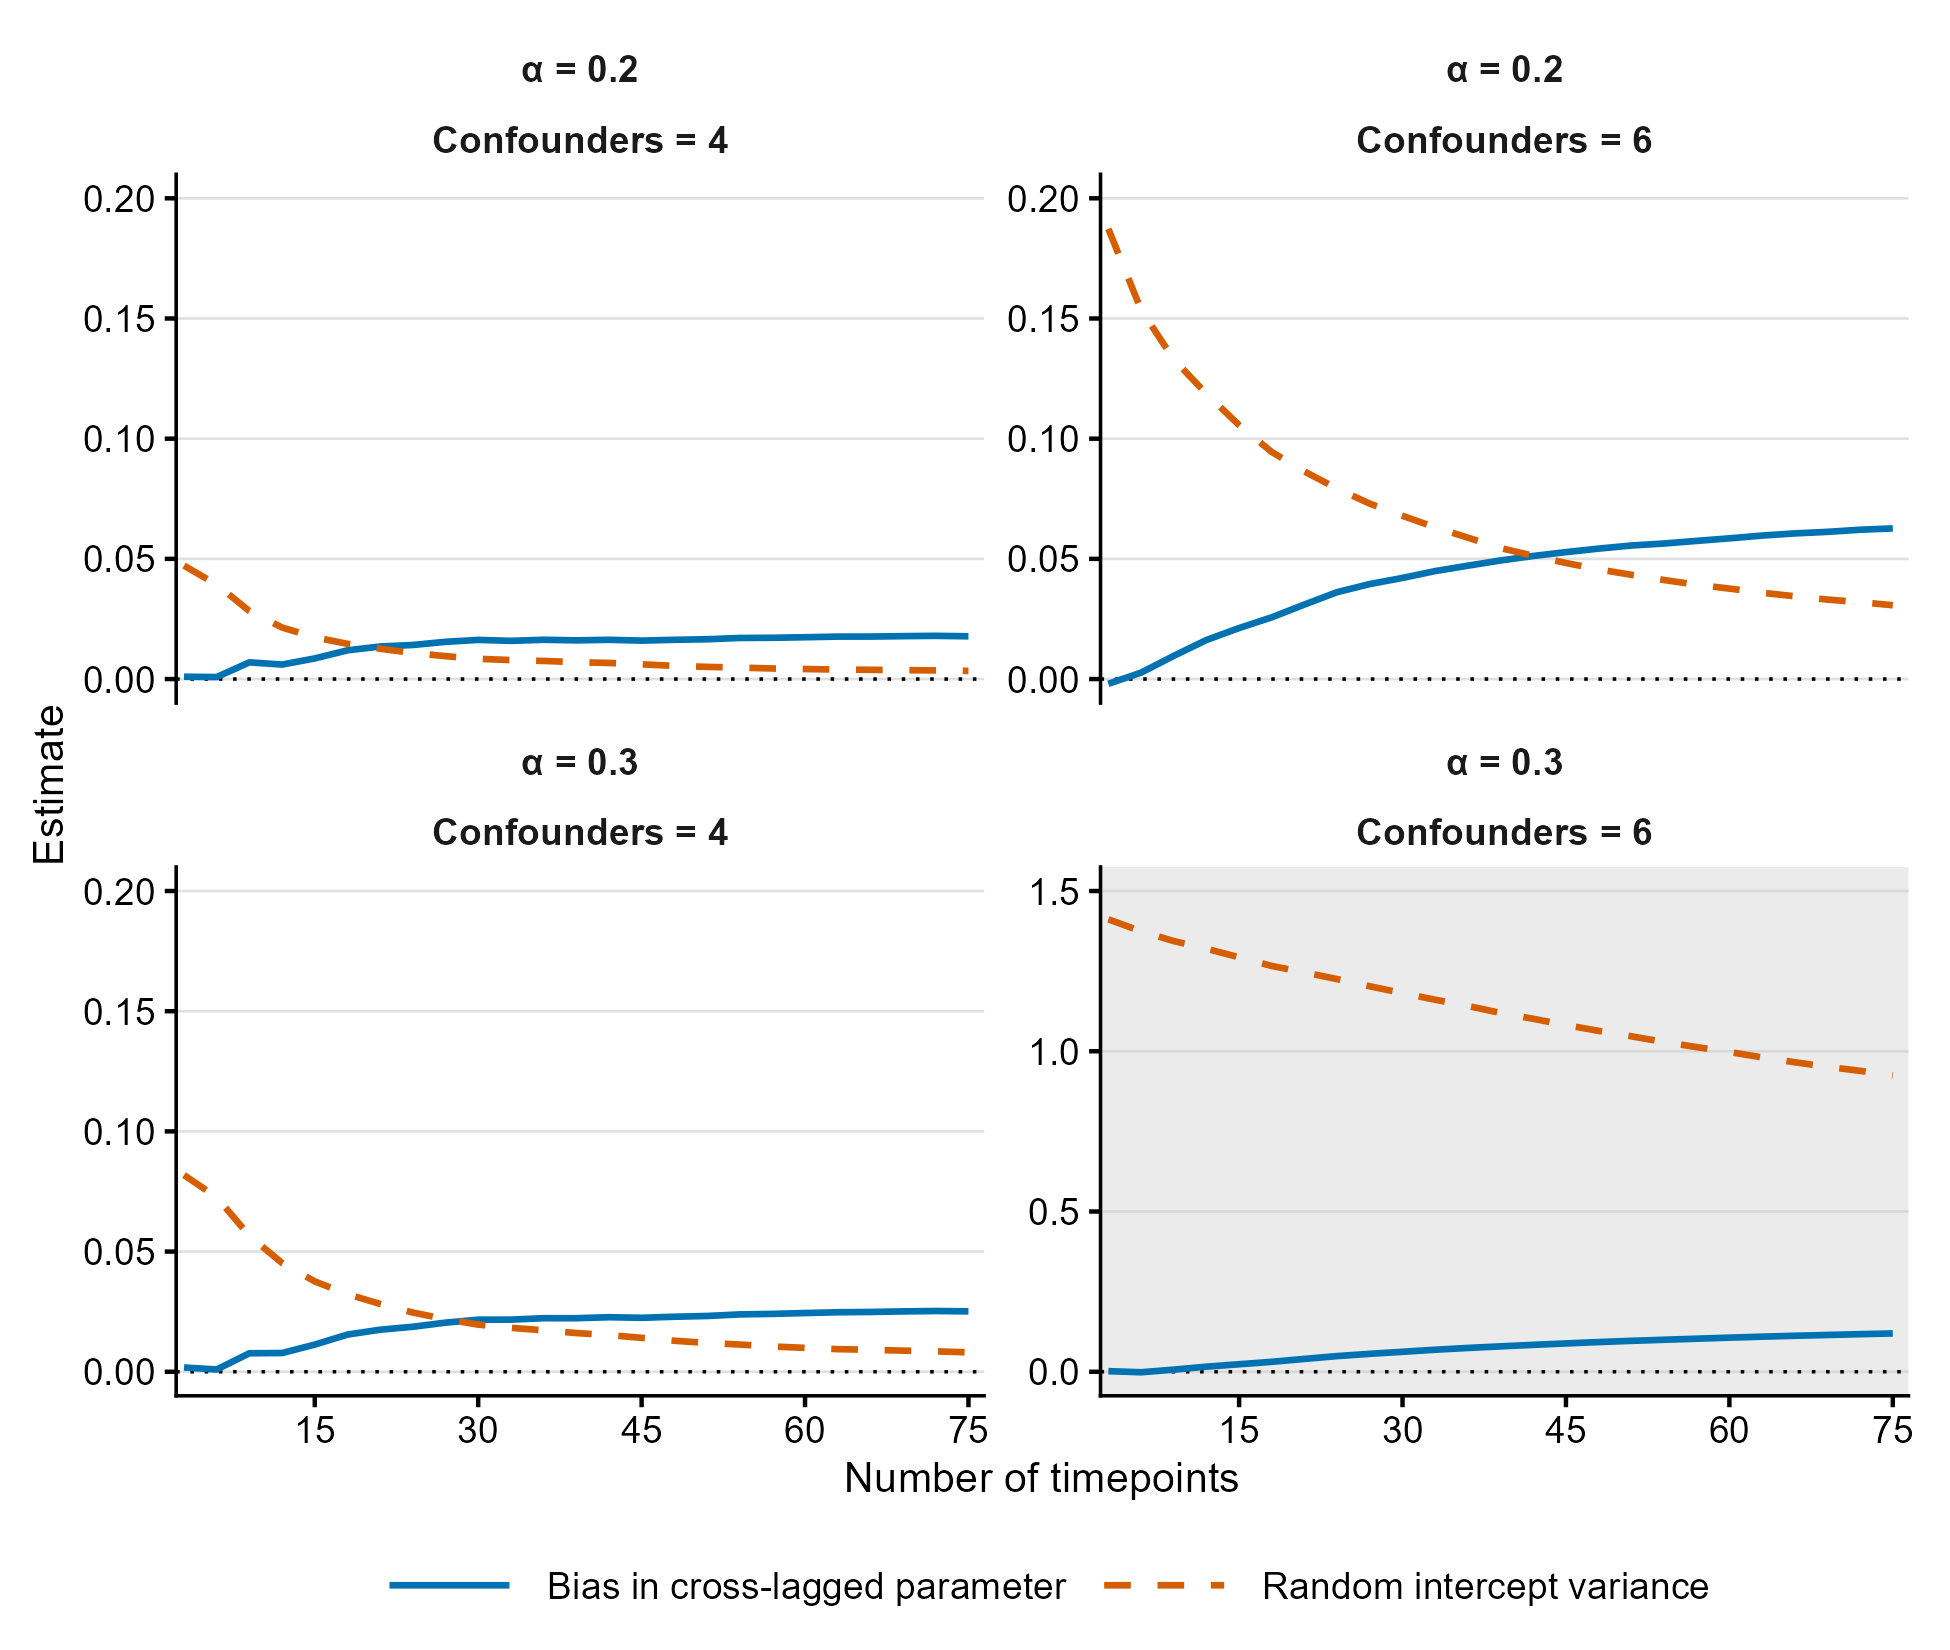
\includegraphics[width=0.7\linewidth,height=\textheight,keepaspectratio]{images/fig_sim1_2x2.png}

\end{figure}%

It is important to note the large increase in illusory trait variance
estimated in the lower-right condition (\(\alpha=.3\) combined with 6
confounders) compared to the other three conditions is due to this
process being close to non-stationarity. Increasing either the number of
confounders to 7 or setting the autoregressive effect to .4 would result
in a process that breaks stationarity.

Concluding, as the number of timepoints increases, the ability of the
RI-CLPM to correct for systems of time-varying confounding deteriorates
as a result of the random intercept failing to capture this confounding
variance. What is striking however, is how well the random intercept is
able to capture this variance on only a small number of timepoints, and
thus allowing the model to retrieve unbiased estimates of the
cross-lagged parameters. This then raises the question if this property
can be exploited for models concerning more timepoints.

\section{The Segmented Random Intercept Cross-Lagged Panel
Model}\label{the-segmented-random-intercept-cross-lagged-panel-model}

In this section we introduce a new model that aims to make use of the
illusory trait finding to correct for time-varying confounding when
there are more than just a few timepoints. The development of this model
is based on the following reasoning: If a random intercept helps to
control~for time-varying confounding across a small number of
timepoints, but fails to do so when the number of timepoints has
increased, one approach could be to estimate multiple random intercepts
on segments (subdivisions) of the total timespan. In this manner, the
new model could be expected to retrieve less biased cross-lagged
parameter estimates, even for data across longer timespans.

\subsection{Model Specification}\label{model-specification}

We propose the Segmented Random Intercept Cross-Lagged Panel Model
(SRI-CLPM), which is a CLPM extended with random intercepts for segments
of the total timespan of the study. Figure~\ref{fig-SRI-CLPM} shows a
schematic example of a SRI-CLPM, specified on segments with two
timepoints.

\begin{figure}[H]

\caption{\label{fig-SRI-CLPM}Schematic representation of the SRI-CLPM.
RI = Random Intercept, all random intercepts are allowed to covary,
represented by the connecting double arrow.}

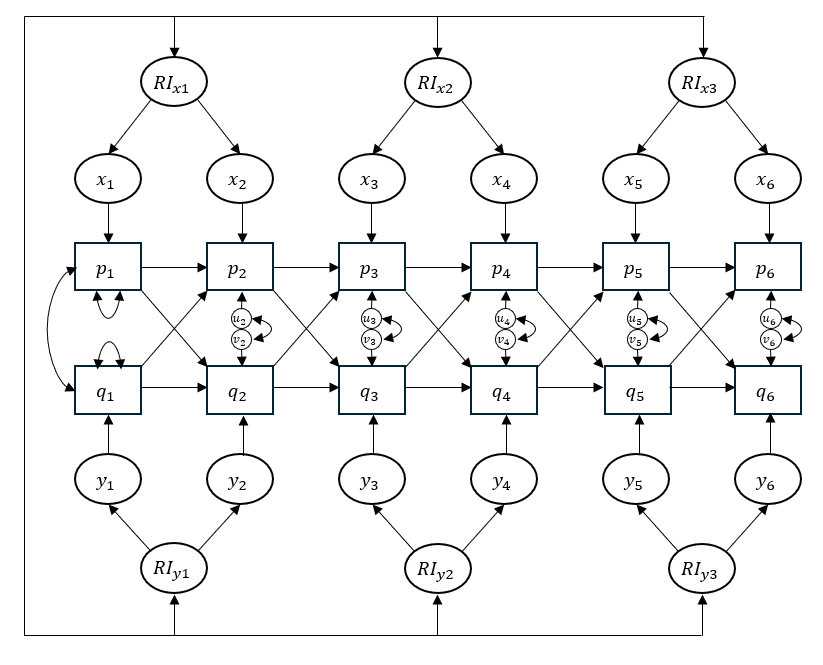
\includegraphics[width=0.8\linewidth,height=\textheight,keepaspectratio]{images/SRI-CLPM.png}

\end{figure}%

The use of the SRI-CLPM requires the user to decide on the segment
length on which a segmented random intercept is specified. Making an
informed decision on the segment length is more challenging than it
might seem at first.~A reasonable expectation is to believe segments of
only two timepoints should yield the least biased estimates, since our
previous results show bias increased when random intercepts are based on
more timepoints. A minimal segment length of two should then work
optimally, if it is identified.~This presupposes however, that
estimating this many latent variables does not introduce unstable
estimation, especially in smaller samples. In addition to this, it is
preferrable to have segments of equal length, and no timepoints should
be left out of a segment. This is important given that we want to be
able to constrain the segmented random intercepts to denote the same
underlying process, something we will explain further in the next
paragraph. Keeping the segments of equal length essentially means the
total number of timepoints should be divisible by the segment length,
once again making the minimum of two an attractive first choice. We
further investigate the effect of segment length with the simulation
presented below.

Another concern is how to estimate the covariance structure of the
latent variables. Imagine a bivariate SRI-CLPM with 30 measurements and
random intercepts estimated on a segment length of two.~ This will
result in 30 separate random intercepts (15 for each repeatedly measured
variable), each with a variance that needs to be estimated. The number
of possible unique covariances between these random intercepts is 465.
Estimating the total latent variable covariance matrix freely thus
results in 495 parameters being estimated for the latent variables
alone. This is much more than the 3 parameters (two variances and a
covariance) that would be included in the standard RI-CLPM for the two
overall random intercepts; it could pose a problem concerning model
parsimony in the best case, and empirical identifiability in the worst
case. Therefore, we choose to impose restrictions on the variances and
covariances between latent variables.

A natural starting point here is to impose constraints that follow the
stationarity assumption along which we also simulate the data. This
implies we constrain the variances of all segmented random intercepts on
the same variable to be equal, since we assume the variance in the
confounding process to be stable over time. In addition, we also
constrain covariances across a set lag to be equal. In our bivariate
example, this would imply two distinct sets of constraints; covariances
between `lateral' random intercepts on the same variable (i.e., two
random intercepts on \(X\)) and covariances between random intercepts on
separate variables (i.e., a random intercept on \(X\) and one on \(Y\)).
Both sets of covariances are constrained to be equal across a set lag,
but both are constrained separately. For example, the covariance between
the first and second random intercepts on \(X\) are constrained equal to
the covariance between the second and third. The same holds for
covariances between a random intercept on \(X\) and one on \(Y\), but
these are not constrained to the same covariance at the same lag on two
random intercepts estimated on the same variable. Constraining the
random intercept covariances in this manner corresponds to a
block-Toeplitz matrix, which can be seen as minimally restrictive
(assuming stationarity) while still reducing the number of parameters
greatly. A schematic representation of the resulting constrained
covariance matrix between the segmented random intercepts can be found
below, alongside the formula for the number of degrees of freedom of a
SRI-CLPM constrained in this manner.

\begin{table}

{\caption{{Constrained segmented random intercept covariance matrix,
shading to illustrate the different `blocks' corresponding to distinct
kinds of covariances.}{\label{tbl-Toep}}}
\vspace{-20pt}}

\begin{center}
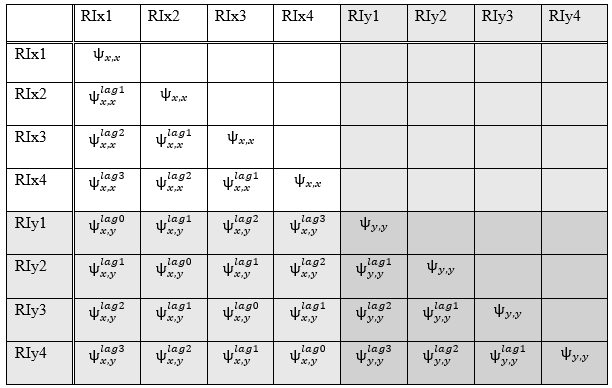
\includegraphics[width=0.9\linewidth,height=\textheight,keepaspectratio]{images/table-toep.png}
\end{center}

\end{table}

The degrees of freedom for a Toeplitz constrained SRI-CLPM can then be
expressed as:

\[
DF=T(2T+1)-(9+4(\frac{T}{SL}-1)+2T)
\]

Where T denotes the number of timepoints and SL denotes the segment
length. Comparing this to the expression for the degrees of freedom of
the unconstrained latent variable covariances below shows the utility of
these constraints.

\[
DF = T(2T+1)-(9+2(\frac{T}{SL})^2+2T)
\]

\subsection{Investigating the Performance of the
SRI-CLPM}\label{investigating-the-performance-of-the-sri-clpm}

Now that we have specified the SRI-CLPM, we evaluate its performance and
behavior with a series of simulation studies. The first is a larger
study aimed at investigating the degree of bias in the cross-lagged
parameters as more timepoints are considered. The second is a more
focused, exploratory study aimed at investigating the statistical power
and type I error rates for cross-lagged parameters as estimated in the
SRI-CLPM.

\subsubsection{Bias in the Cross-Lagged
Parameters}\label{bias-in-the-cross-lagged-parameters}

In order to evaluate the degree of bias in the cross-lagged parameters
retrieved by the SRI-CLPM, we perform a Monte Carlo simulation. Once
again, we generate data according to the data generating mechanism
described in Bailey et al.
(\citeproc{ref-baileyIllusoryTraitsWrong2024}{2024}), corresponding to a
CLPM with systems of time-varying confounding. Similar to the first
simulation, we choose to estimate models on differing numbers of
timepoints to evaluate the performance of the model as more timepoints
are considered. But in contrast to the first simulations, we make use of
smaller, more realistic sample sizes (i.e., 250 and 500 cases) to assess
the practical utility for researchers. We make use of 3000 replications
in each condition~to study sampling variation, allowing us to retrieve
empirical sampling distributions for the model parameters.

The study length that we consider was chosen to be 6, 12, 18, 24 and 30
timepoints. This is done so all numbers of timepoints can be divided by
both 2 and 3, allowing us to specify segments of these lengths. In this
manner we aim to get some indication of the role of segment length in
the performance of the model. To assess the performance of the
Toeplitz-constrained random intercept covariances we estimate two
specifications of the SRI-CLPM: one with these constraints and one with
freely estimated random intercept variances and covariances.

Figure~\ref{fig-boxplots} shows the distributions of one of the
cross-lagged parameter estimates, visualized as boxplots, as they are
obtained from various models and for an increasing number of timepoints.
The true parameter value is .1, displayed as the horizontal dotted line.
The RI-CLPM's cross-lagged parameter estimates slowly increase to the
uncorrected biased estimates retrieved by the CLPM. As expected, the
SRI-CLPM is able to retrieve less biased cross-lagged parameter
estimates when the number of timepoints considered increases, at the
cost of somewhat larger variance in the sampling distribution compared
to the CLPM and RI-CLPM. Figure~\ref{fig-boxplots} also shows the effect
of the segment length chosen for the random intercepts has on the bias
and sampling variability of the cross-lagged parameters. Increasing the
segment length from two to three leads to a slight increase in bias, but
in turn also reduces sampling variability slightly, which is likely due
to the decrease in the number of parameters estimated that needs to be
estimated when the segment is larger.~

\begin{figure}[H]

\caption{\label{fig-boxplots}Sample distributions of the cross-lagged
parameter per model specification. Boxplots represent the interquartile
range of point estimates. Dashed line represents the true value of .1.
SL = segment length, -free indicates the model had freely estimated
covariances between segmented random intercepts.}

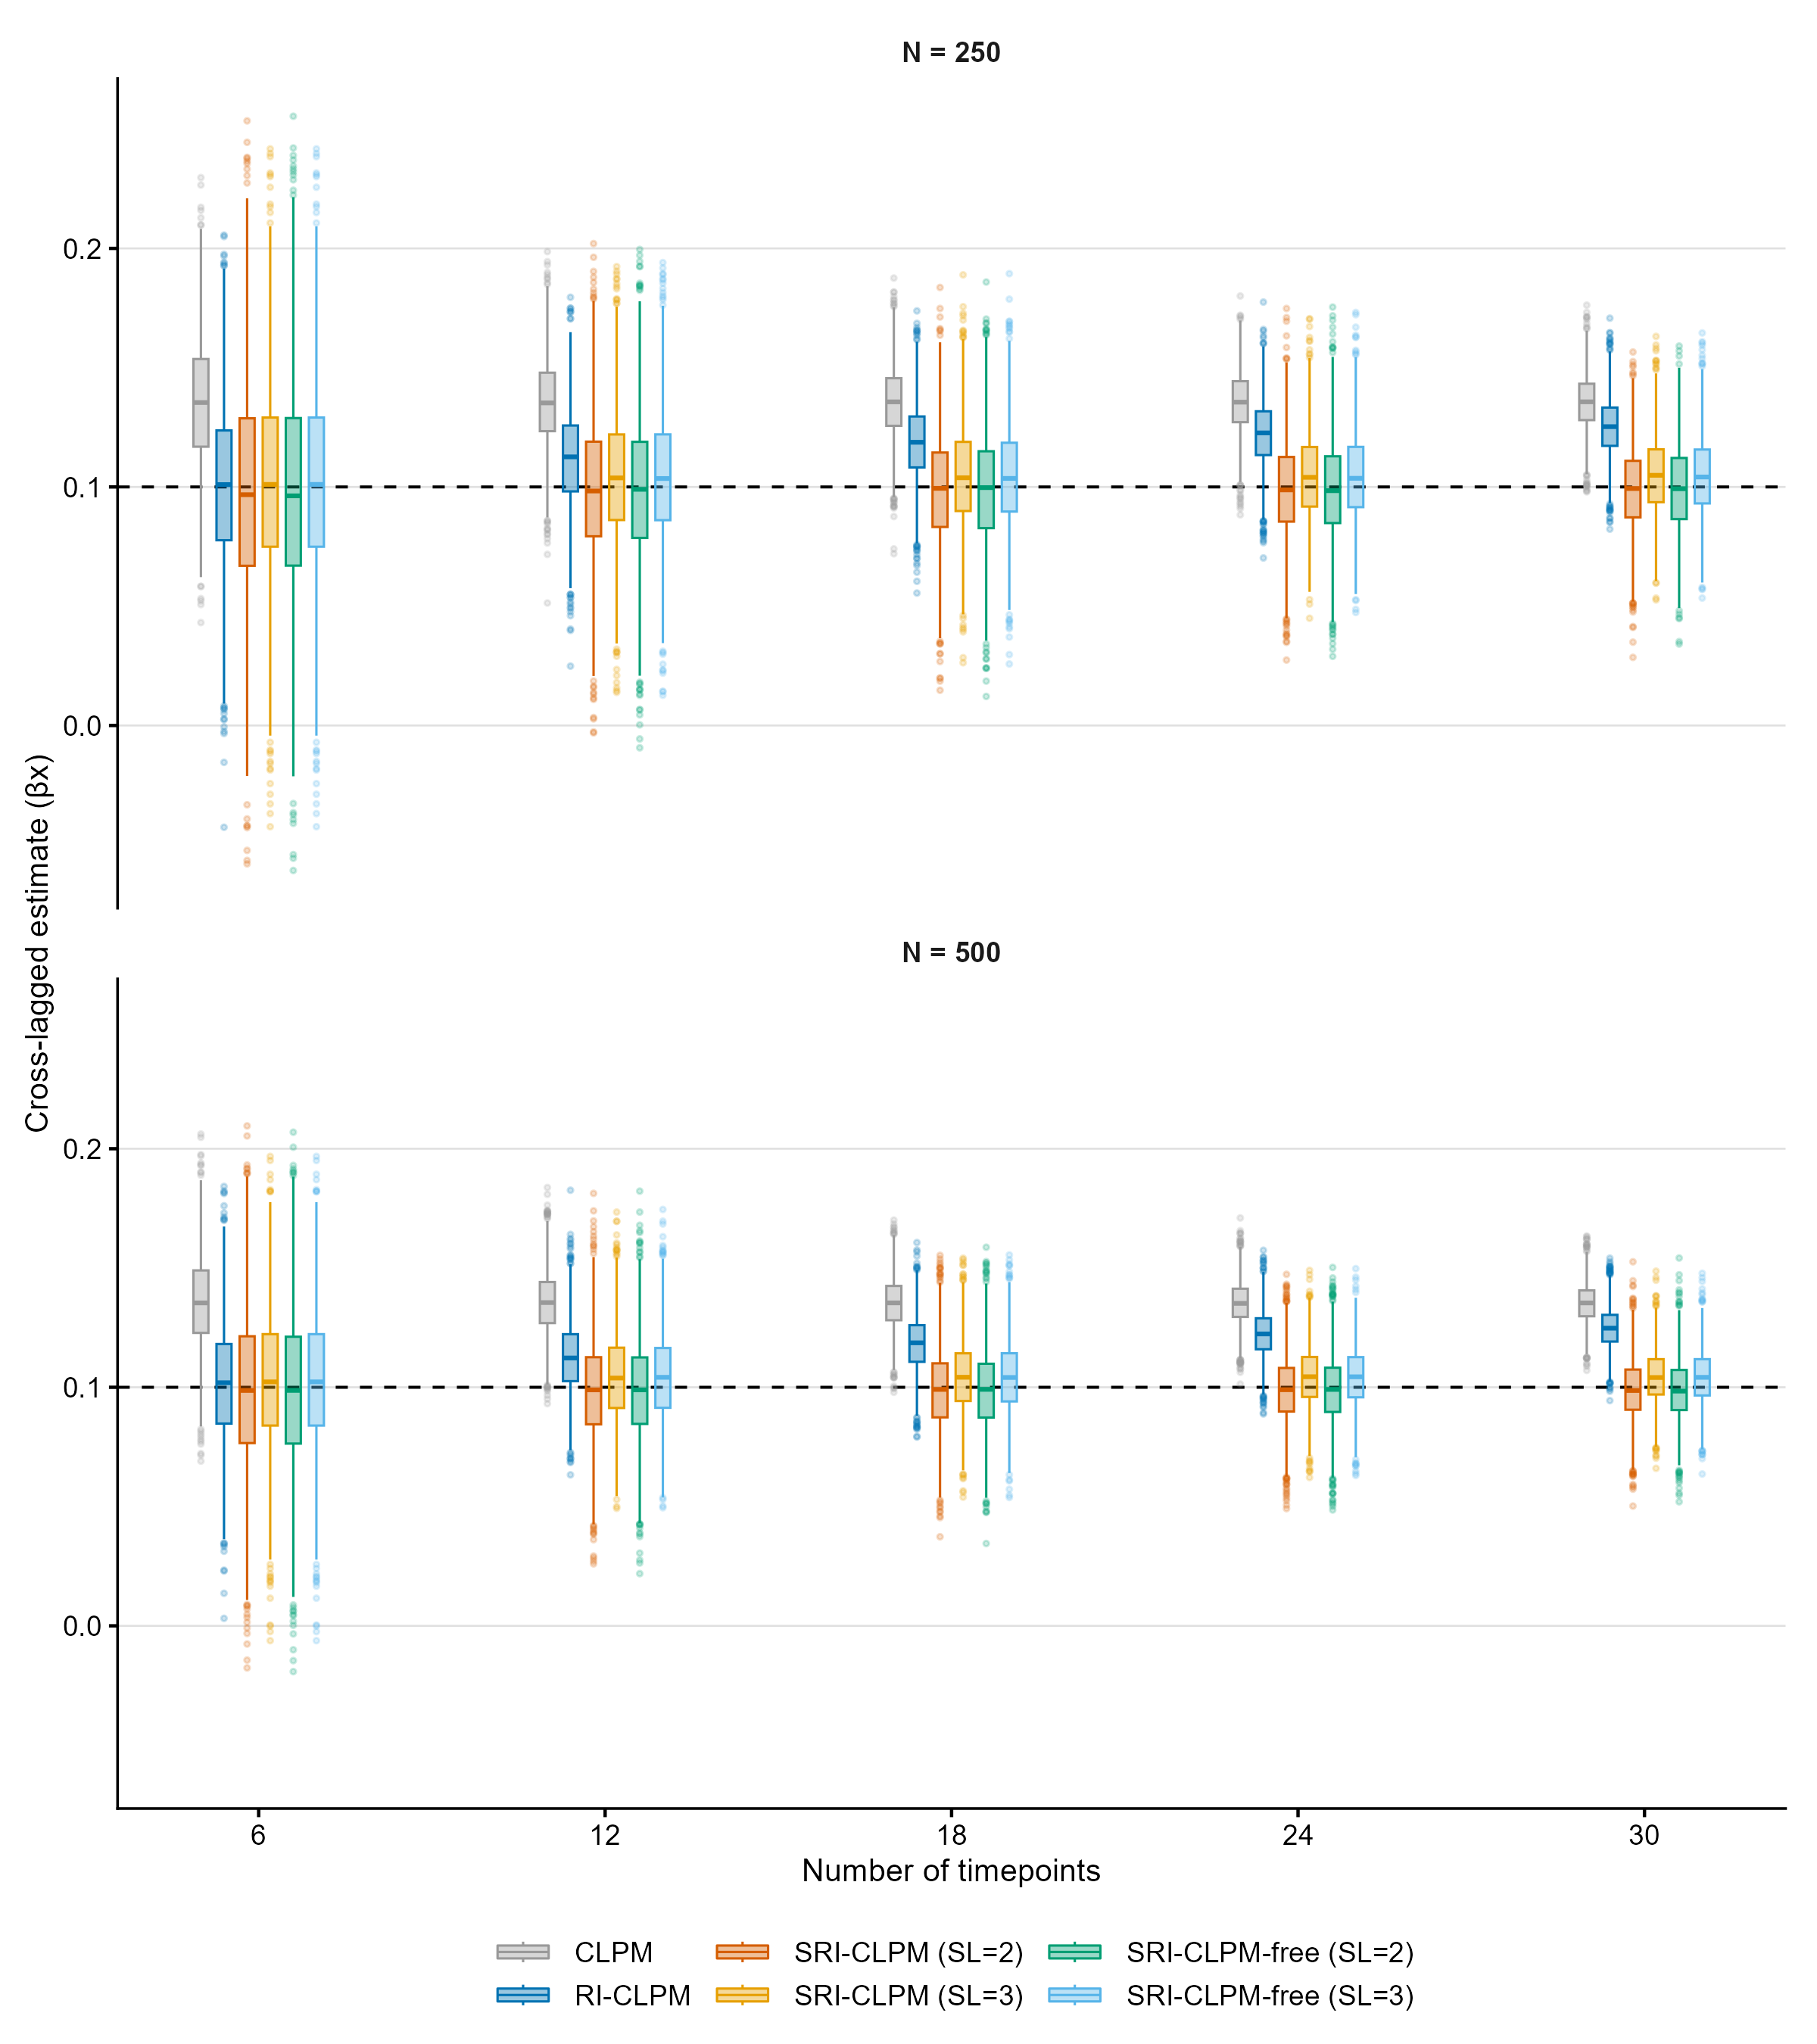
\includegraphics[width=1.05\linewidth,height=\textheight,keepaspectratio]{images/fig_T_effect_bx.png}

\end{figure}%

Figure~\ref{fig-heatmap} shows the 95\% confidence interval coverage
rates for all structural parameters (also including the autoregressive
parameters), comparing the SRI-CLPM (right column) with Toeplitz latent
variable constraints and a segment length of 2 to the CLPM (left column)
and RI-CLPM (middle column). The coverage rates for cross-lagged
parameters show a substantial improvement over the biased estimates in
the RI-CLPM and CLPM. Interestingly however, the autoregressive
parameters show a marked decline in 95\% CI coverage rates as more
timepoints are considered. Another puzzling aspect of this is that it
seems the model decline is more pronounced on the larger sample size,
which is somewhat alarming. It is important to note however, that
retrieving unbiased estimates of autoregressive parameters was not the
goal of this simulation and is usually not the goal of cross-lagged
panel modeling.

\begin{figure}[H]

\caption{\label{fig-heatmap}Heatmap showing the 95\% confidence interval
coverage rates for all structural parameters per model, per timepoint
and per sample size condition (N). Coverage rate denotes the frequency
with which the true value was contained in the 95\% confidence
interval.}

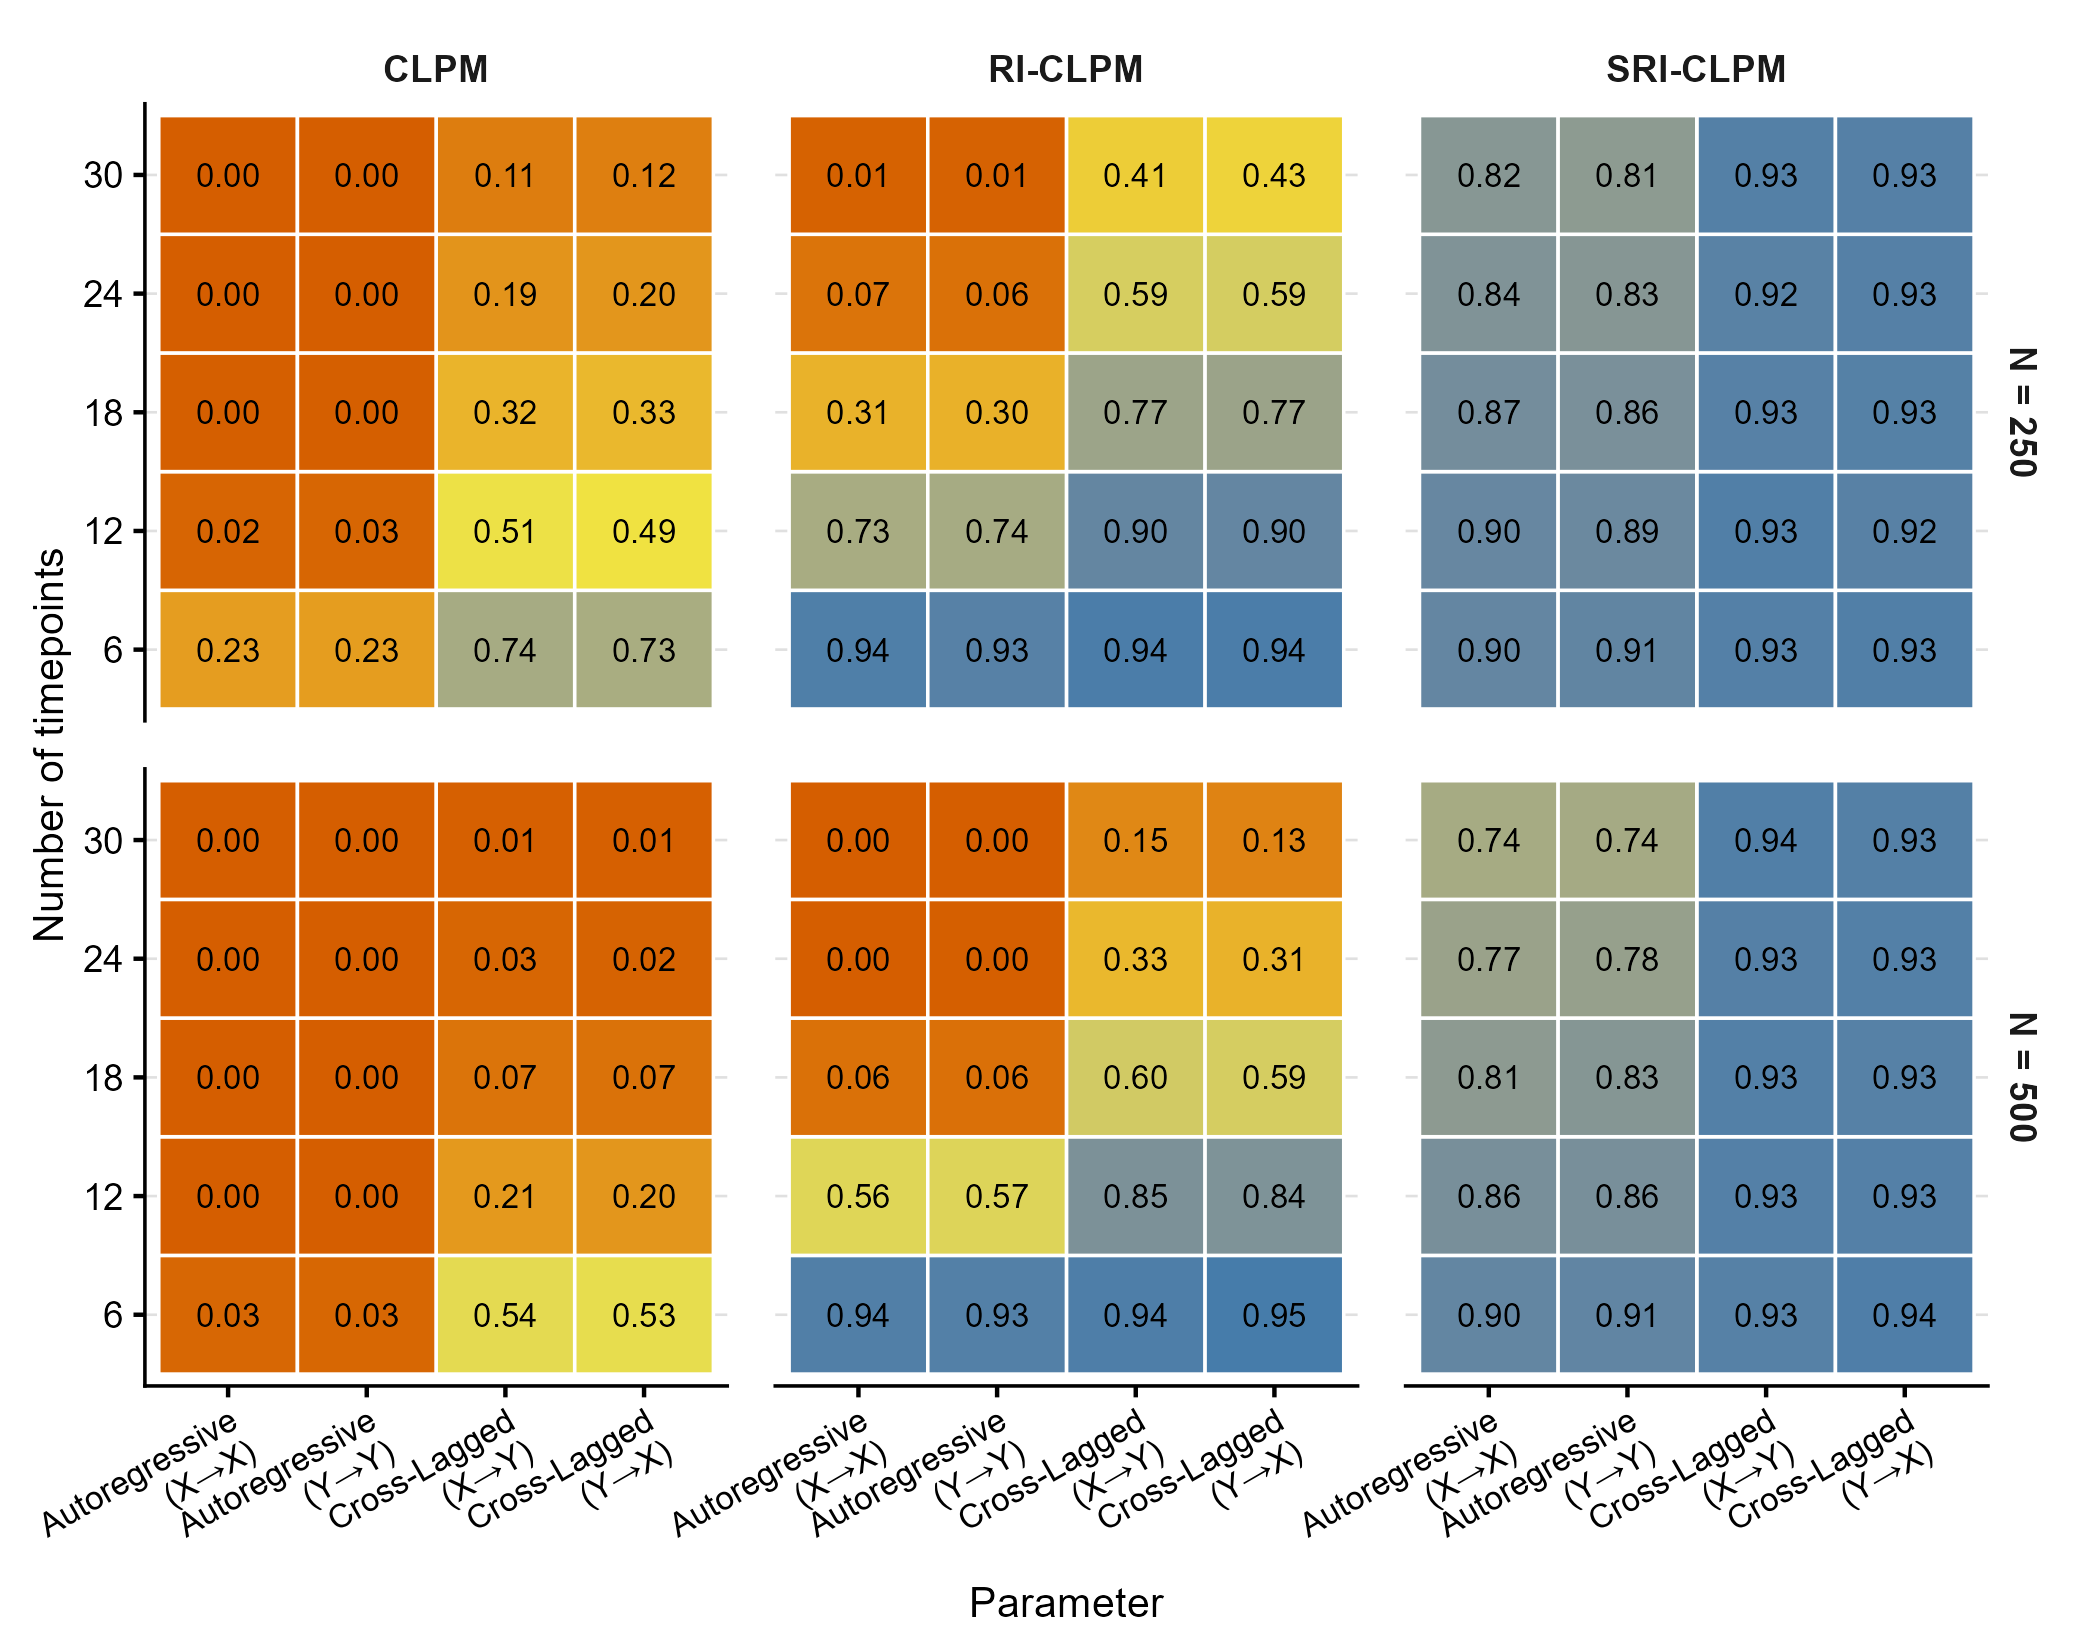
\includegraphics[width=1\linewidth,height=\textheight,keepaspectratio]{images/fig_coverage_heatmap.png}

\end{figure}%

\subsubsection{Investigating Statistical Power and Type I Error with the
SRI-CLPM}\label{investigating-statistical-power-and-type-i-error-with-the-sri-clpm}

We present an additional simulation study aimed at investigating the
statistical power and type I error rates for the cross-lagged parameters
as estimated in the SRI-CLPM. To achieve this, we generate data from the
same mechanism as before, only setting one of the cross-lagged effects
to zero. This allows us to assess both statistical power in detecting
the true cross-lagged effect of .1, and the type I error rate of
detecting an effect when the true cross-lagged effect is zero. For
simplicity, we focus on 20 timepoints, using a segment length of two,
while varying the sample sizes between 100, 150 and 200. For each of
these three conditions, we simulated a thousand replications.

The distribution of p-values for the cross-lagged parameters are
presented in Figure~\ref{fig-power} below, along with the statistical
power and type I error. The SRI-CLPM shows acceptable power on samples
as small as 100 cases and a relatively uniform p-value distribution on
the cross-lagged effect that was set to zero. There is however a
somewhat inflated type I error rate when compared to the nominal
\(\alpha\) of .05 used, which importantly does decrease on larger sample
sizes.

\begin{figure}[H]

\caption{\label{fig-power}Distributions of estimated p-values per
cross-lagged parameter true value (0.1 or 0) per sample size condition
(N). Bar chart shows the distributions, power denotes the percentage
where the null hypothesis was correctly rejected, type I error denotes
the percentage where the null hypothesis was incorrectly rejected.}

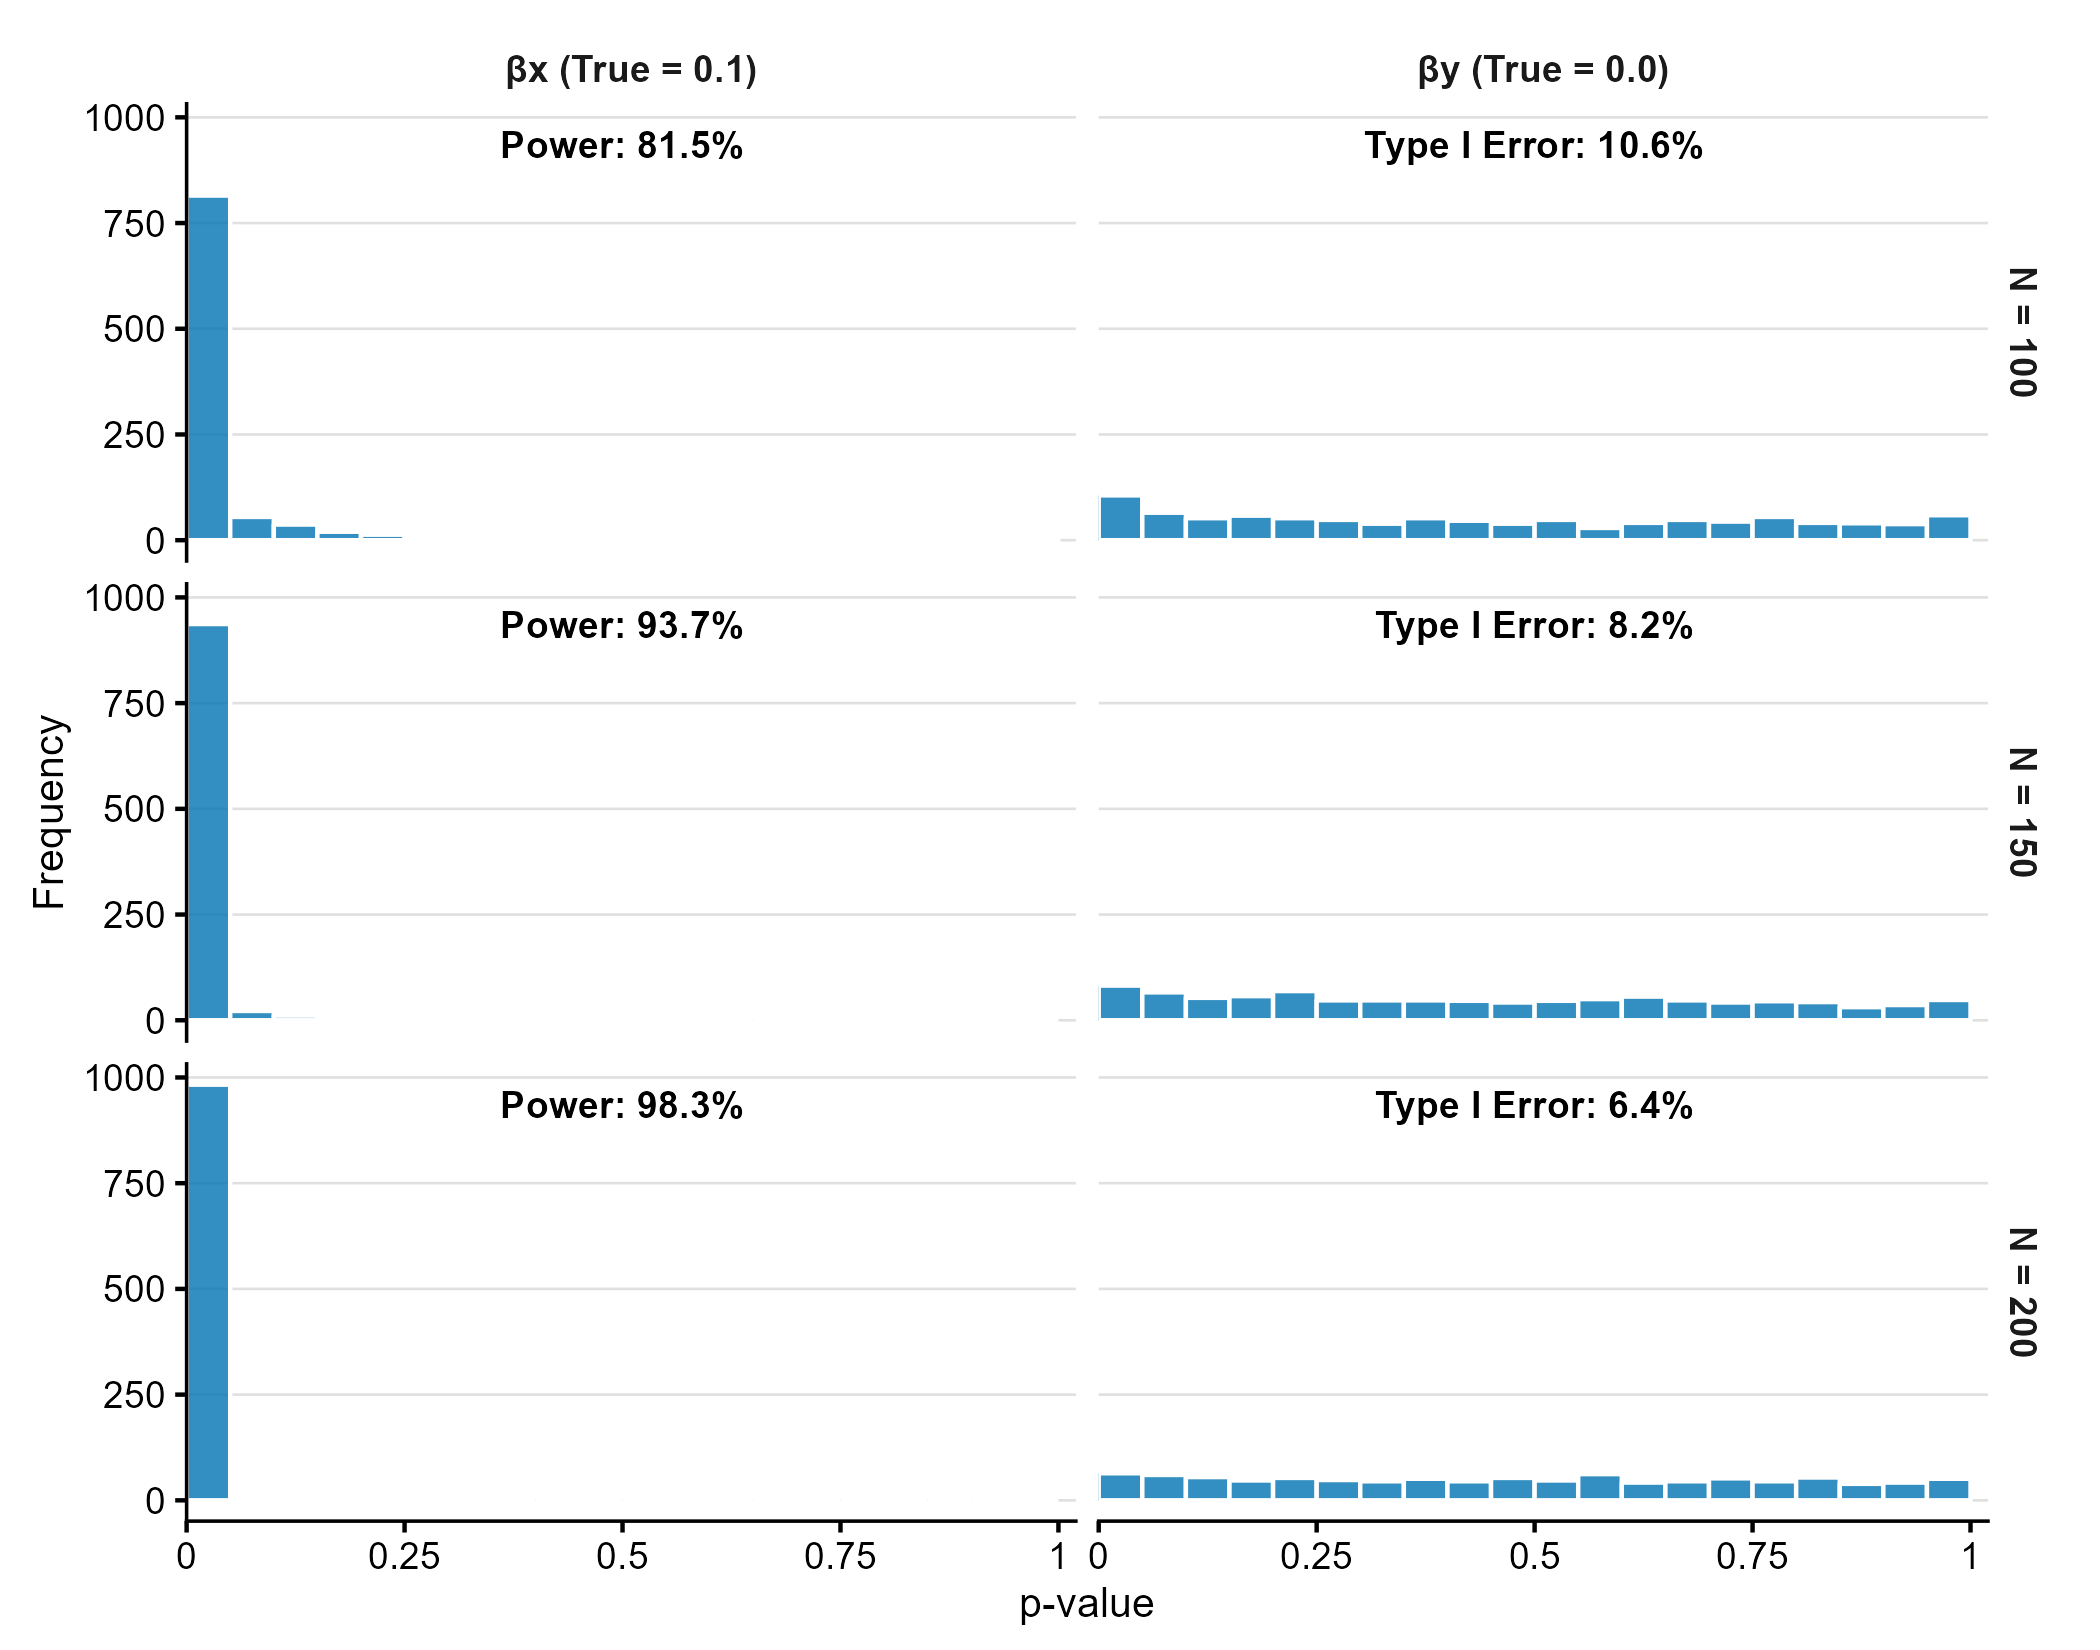
\includegraphics[width=0.8\linewidth,height=\textheight,keepaspectratio]{images/fig_power.png}

\end{figure}%

It is important to note that during the estimation of the SRI-CLPM's the
covariance matrix of latent variables is often not positive definite.
Additionally, lavaan also incidentally reports the variance-covariance
matrix of the estimated parameters to not be positive definite. On
inspection of an estimated correlation matrix for a SRI-CLPM with freely
estimated latent variable covariances, we found that adjacent segmented
random intercepts are structurally estimated to be correlated higher
than 1. This reflects an improper solution found by the estimator;
possibly indicating a structural problem with empirical identifiability.
This problem persists even if models are fitted on very large amounts of
data (50.000 cases) and using the Toeplitz-constraints. For now we have
reported the estimated cross-lagged parameters, since these do not seem
to be anomalous, and will comment more on estimation in the discussion.

Concluding, the SRI-CLPM is able to retrieve less biased estimates of
the cross-lagged parameters when the number of timepoints increases
compared to the RI-CLPM and CLPM. This comes at the cost of somewhat
larger standard errors, yet acceptable statistical power in the
condition we simulated. The Toeplitz-constrained covariances between the
random intercepts work well for the stationary, ergodic process used,
with the choice of segment length

\section{The SGRI-CLPM}\label{the-sgri-clpm}

Until now, we have only considered processes containing systems of
time-varying confounding, introducing the SRI-CLPM to control for its
influence. We therefore have the RI-CLPM, designed to control for
time-invariant confounding and the SRI-CLPM, designed for controlling
for time-varying confounding. This raises the question however, to what
extent the SRI-CLPM is able to control for time-invariant confounding or
a combination of both types of confounding. Additionally, it might be
interesting to see whether it is possible to separate the confounding
variance into a time-varying and time-invariant component, allowing
researchers to get an idea of the source of the confounding. We
therefore in this section introduce the idea of adding a `global' random
intercept to the SRI-CLPM, aimed at capturing time-invariant
confounding. The motivation for this is simple: We expect there to be
substantial time-invariant confounding in any process of interest,
especially concerning person-to-person differences in the social
sciences. Therefore, a model which could correct for the influence of
both types of confounding while accurately partitioning their associated
variance would be an asset.

\subsection{Model Specification}\label{model-specification-1}

Aiming to capture time-invariant confounding, we specify a variation of
the SRI-CLPM with the addition of a global random intercept estimated on
all repeated measurements of a variable, resembling the standard
RI-CLPM. These global random intercepts can be allowed to covary freely,
but are assumed to be independent of the other segmented random
intercepts. In this manner, we hope to be able to distinguish variance
associated with time-invariant confounding from variance associated with
time-varying confounding. A schematic representation of this new model,
which we refer to as the SGRI-CLPM, is shown in
Figure~\ref{fig-SGRI-CLPM} below.

\begin{figure}[H]

\caption{\label{fig-SGRI-CLPM}Schematic representation of the SGRI-CLPM.
RI = random intercept, GRI = global random intercept. Random intercepts
are allowed to covary, but their covariance with the global random
intercepts is constrained to zero.}

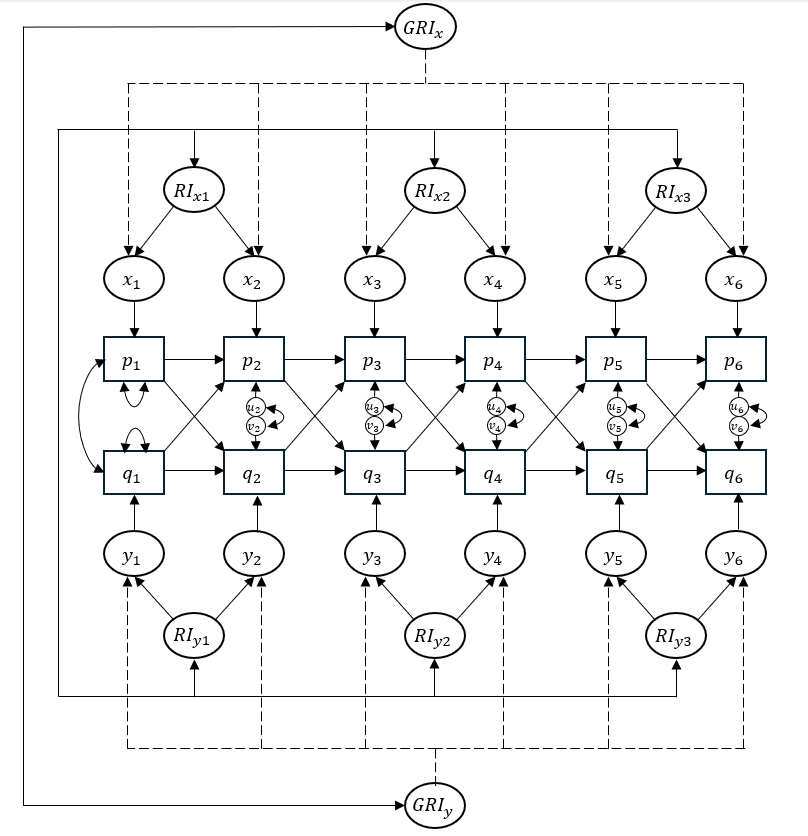
\includegraphics[width=0.7\linewidth,height=\textheight,keepaspectratio]{images/SGRI-CLPM.png}

\end{figure}%

\subsection{Investigating Cross-Lagged Parameter Bias in the
SGRI-CLPM}\label{investigating-cross-lagged-parameter-bias-in-the-sgri-clpm}

We assess the performance of the SGRI-CLPM with another Monte Carlo
simulation study, comparing it to the performance of the SRI-CLPM. For
this, the data generating mechanism introduced by Bailey et al.
(\citeproc{ref-baileyIllusoryTraitsWrong2024}{2024}) is extended to also
allow for the generation of data with time-invariant confounding. We
assume the time-invariant confounding is orthogonal to the time-varying
confounding, meaning we only have to generate a between-case deviation
from the mean. This entails specifying a variance for both the
confounder on \(X\) and on \(Y\), taking into account their covariance.
Afterwards, this deviation from the mean per case can be added to its
time-varying process.

Both the SRI-CLPM and this extended SGRI-CLPM~are then used to analyze
the data generating with various mechanisms: either with only
time-varying confounding or with both types of confounding. Both
specifications use the Toeplitz-constrained segmented random intercept
covariances and a segment length of three, on 30 total timepoints. While
earlier simulations show a smaller segment length yielding better
results, three was chosen as a convenient way to divide 30 timepoints.
We simulate 1000 replications, using a realistic sample size of 200. The
distributions of cross-lagged parameter estimates for the two model in
each of the conditions are plotted in Figure~\ref{fig-SGRIboxplot}.
Interestingly, the model specifications seem to perform identically at
retrieving unbiased cross-lagged parameter estimates, even when a
time-invariant component is added. This becomes especially clear in
Figure~\ref{fig-scatter}, where the point estimate of the SGRI-CLPM is
plotted against the point estimate of the SRI-CLPM on the same data,
which shows that these are virtually identical.

\begin{figure}[H]

\caption{\label{fig-SGRIboxplot}Interquartile ranges for estimated
cross-lagged parameters per model, per confounding condition. Dashed
line represents the true value of .1.}

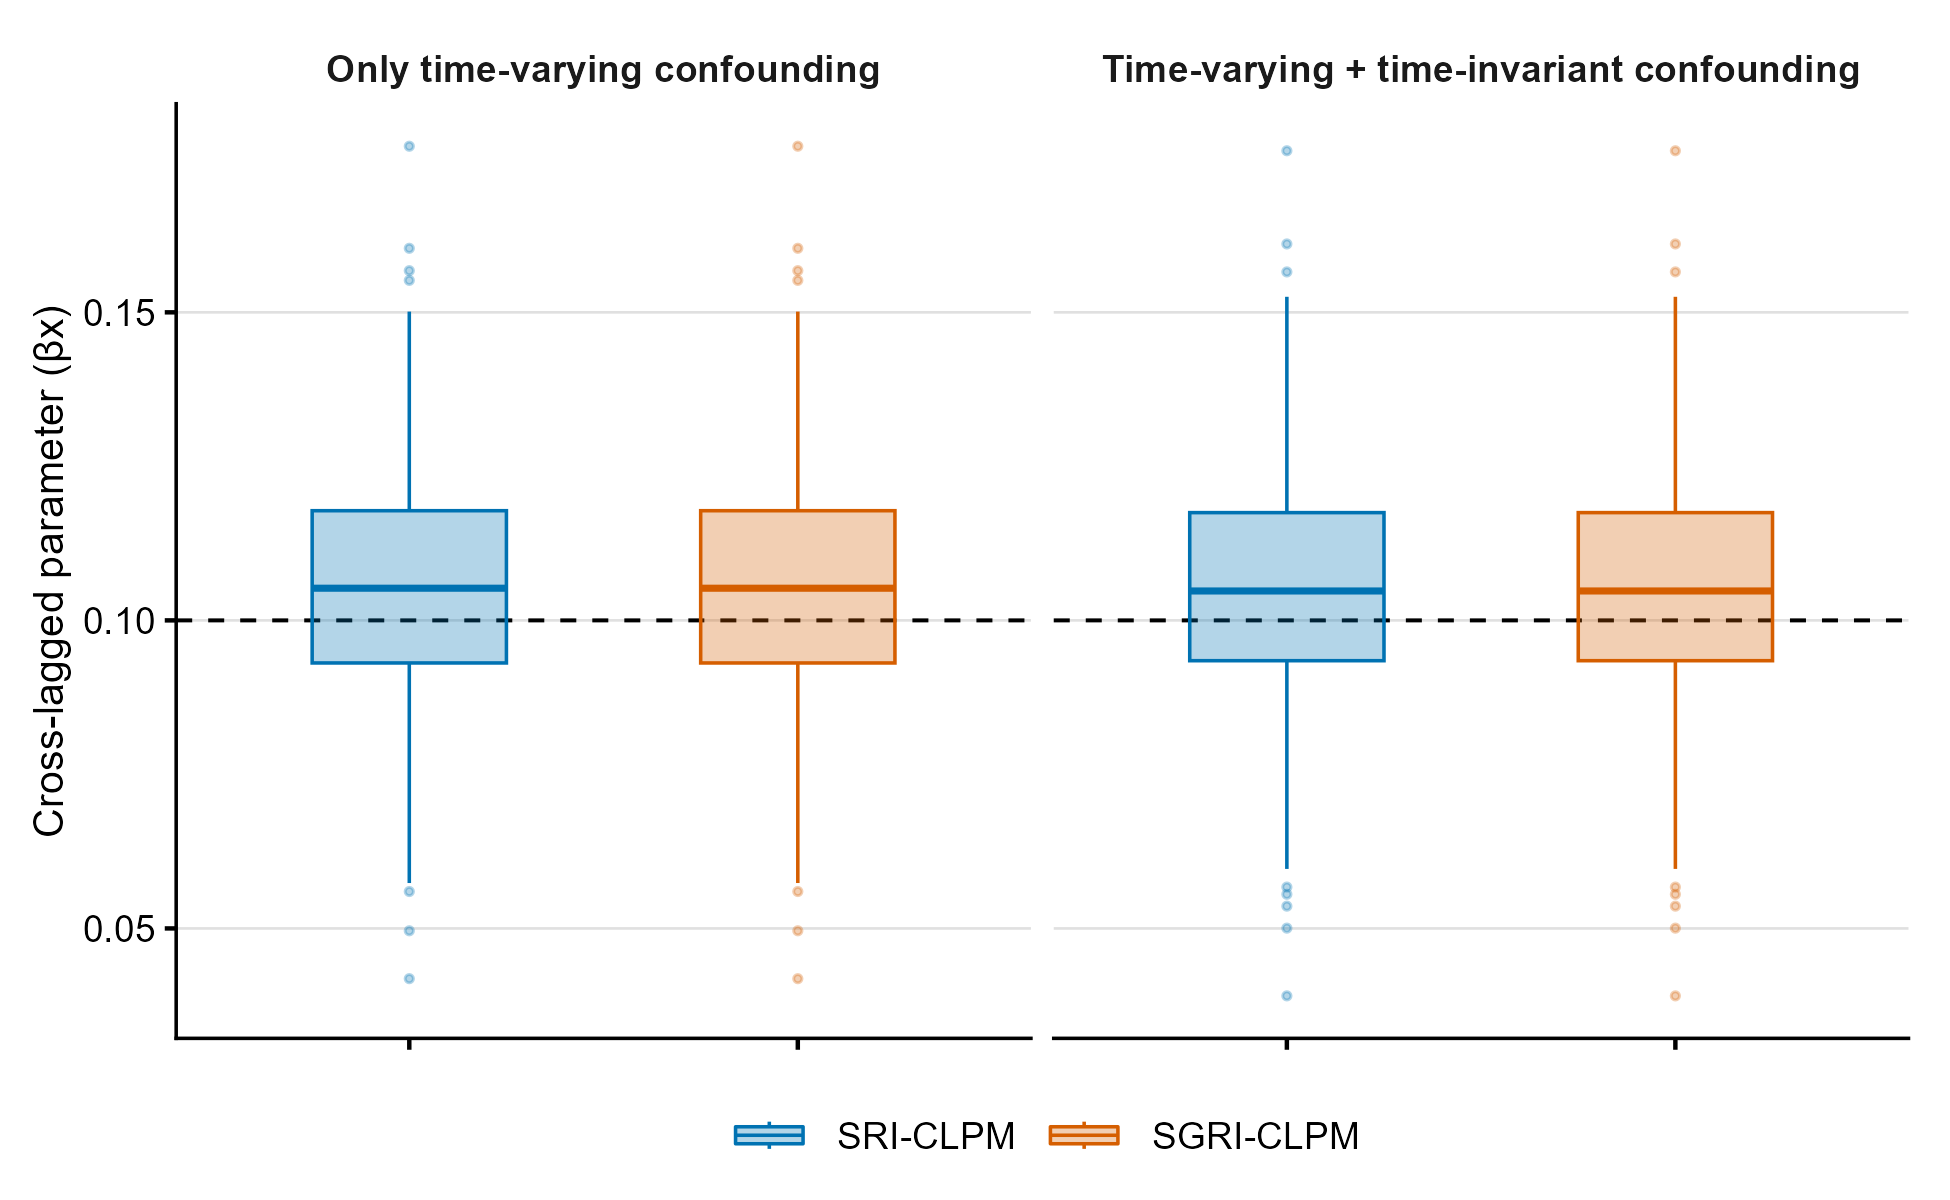
\includegraphics[width=0.6\linewidth,height=\textheight,keepaspectratio]{images/fig_srig_comparison.png}

\end{figure}%

\begin{figure}[H]

\caption{\label{fig-scatter}Point estimates for both model
specifications on the same data plotted against one another, per
confounding condition. Dashed line represents equality between both
estimates.}

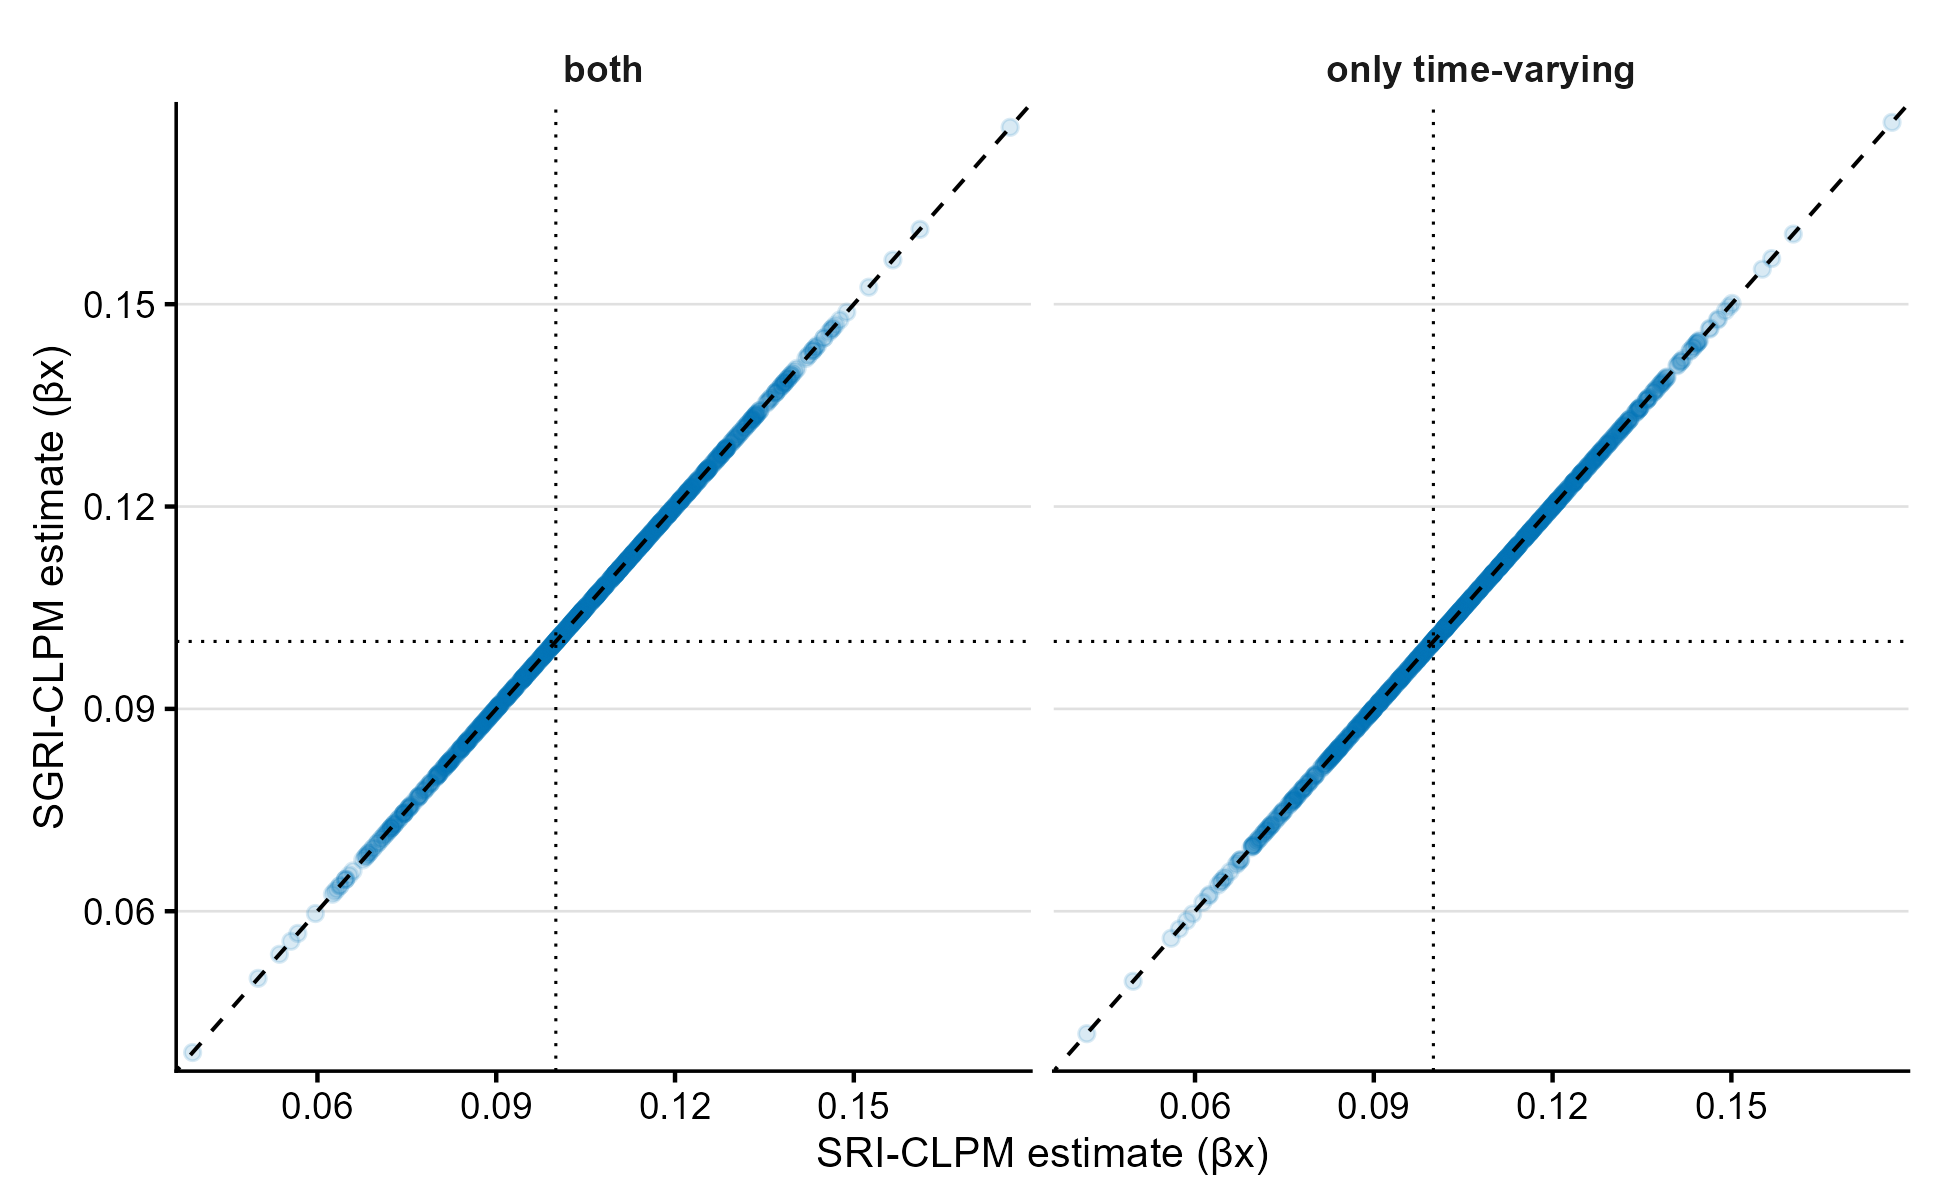
\includegraphics[width=0.6\linewidth,height=\textheight,keepaspectratio]{images/fig_scatter.png}

\end{figure}%

Hence, the only potential added benefit of a global random intercept may
be its alleged ability to partition confounding variance into a
time-varying and time-invariant component. To assess this ability we
should look at the estimated global random intercept variances and their
associated covariance.

\subsection{Random Intercept Variances in the
SGRI-CLPM}\label{random-intercept-variances-in-the-sgri-clpm}

The SGRI-CLPM estimates two random intercept variances per variable of
interest, assuming all the segmented random intercept variances are
constrained to be equal. We estimate a global random intercept variance
representing a stable, time-invariant confounding component and a
segmented random intercept variance representing fleeting, time-varying
confounding. We have already seen that adding the segmented random
intercepts is sufficient for correcting for the influence of both
time-varying and time-invariant confounding on the estimation of
cross-lagged parameters. However, researchers might also be interested
in uncovering the source of the confounding, to which end separating the
time-varying and time-invariant components could be useful.

To assess how accurately the SGRI-CLPM can separate the confounding
variance into the time-varying and time-invariant components, we
generate data with all four combinations of confounding. This means we
generate data according to a simple CLPM without confounding, a CLPM
with time-varying confounding, a CLPM with time-invariant confounding
(i.e., RI-CLPM) and a CLPM with both types of confounding. We can then
compare the estimated segmented random intercept variance and the global
random intercept variance across these conditions. All conditions are
replicated 500 times, with a sample size of 200 and using a SGRI-CLPM
estimated on 20 timepoints with a segment length of two. It should be
noted at this point that the values for the segmented random intercept
and global random intercept cannot be directly compared. The global
random intercept variance is attributed to one underlying latent
variable, indicated by all measurements and should therefore in theory
retrieve the variance specified for the time-invariant component in the
data generating mechanism. In contrast, the segmented random intercept
variance is constrained to be equal across multiple latent variables,
each having an effect on a segment of the total timespan. The estimated
segmented random intercept variance therefore does not necessarily
retrieve one inputted variance in the data generating mechanism.

Table~\ref{tbl-sgri-summary}~shows the mean random intercept variances
of \(X\) per condition, alongside the mean point estimate of the
cross-lagged parameter of \(X\) on \(Y\). When the unconfounded CLPM
generated the data, the SGRI-CLPM correctly estimate random intercept
variances around 0 for both the segmented and global random intercepts,
but it does suffer from improper solutions by estimating negative
variances. Interestingly, the global random intercept seems to be able
to capture the stable component relatively well. In the conditions where
a time-invariant confounder was present (time-invariant and combined)
the mean estimate is relatively close to the true value of 1. There does
seem to be some misattribution of variance into the other components,
which is most clearly visible in the time-invariant condition. We would
expect the global random intercept to capture the complete confounding
variance of 1, yet a small portion of the variance is attributed to the
segmented random intercepts. The same holds for the time-varying
condition, although the difference here is harder to interpret because
we have not quantified the total time-varying component. The combined
condition shows a promising separation, although the time-varying
component seems to be somewhat inflated.

\begin{table}

{\caption{{Mean of Point Estimates for SGRI Model Parameters Across
Simulation Conditions}{\label{tbl-sgri-summary}}}
\vspace{-20pt}}

\begin{longtable*}[t]{lrrr}
\toprule
Condition & Global RI & Segmented RI & Cross-Lagged Parameter\\
\midrule
\cellcolor{gray!10}{Pure (No Confounding)} & \cellcolor{gray!10}{-0.008} & \cellcolor{gray!10}{0.008} & \cellcolor{gray!10}{0.102}\\
Time-varying & 0.034 & 0.041 & 0.100\\
\cellcolor{gray!10}{Time-invariant} & \cellcolor{gray!10}{0.968} & \cellcolor{gray!10}{0.026} & \cellcolor{gray!10}{0.101}\\
Combined & 1.010 & 0.059 & 0.099\\
\bottomrule
\end{longtable*}

\end{table}

These results should be seen as exploratory, and a proof of concept.
Further work is needed to validate the SGRI-CLPM's ability to separate
confounding into its source components. We only show here that it is in
theory possible to make some sort of separation, whether this separation
can be made cleanly and accurately cannot be said from this simulation
alone. If a researchers only interest is to control for the influence of
unobserved confounding, whether time-varying or time-invariant, the
SRI-CLPM suffices.

\newpage

\section{Discussion}\label{discussion}

In this paper, we aim to apply the `illusory trait' finding as presented
by Bailey et al. (\citeproc{ref-baileyIllusoryTraitsWrong2024}{2024}) to
control for time-varying confounding in cross-lagged panel modeling when
the number of timepoints increases. Unobserved confounding is a serious
threat to the estimation of structural parameters in SEM
(\citeproc{ref-hamakerCritiqueCrosslaggedPanel2015}{Hamaker et al.,
2015}; \citeproc{ref-murayamaThinkingClearlyTimeinvariant2024}{Murayama
\& Gfrörer, 2024};
\citeproc{ref-rogosaCritiqueCrosslaggedCorrelation1980}{Rogosa, 1980}).
While theoretically identifying possible confounders and controlling for
their influence through their modeling as covariates may be considered
preferable, it is unlikely that we are able to always observe all
potential confounders. We therefore introduced a new model we refer to
as the Segmented Random Intercept Cross-Lagged Panel Model (SRI-CLPM),
which consists of extending the CLPM with random intercepts for segments
of the total study duration. Simulation results show the SRI-CLPM
successfully controls for confounding, whether time-varying,
time-invariant, or both. We believe a model that is able to retrieve
unbiased cross-lagged parameters regardless of the presence or absence
of any type of confounding to be of substantive interest to researchers.

In the first simulation, we have shown that the illusory random
intercept variance decreases as the number of timepoints increases. As a
result, the ability of the RI-CLPM to retrieve less biased estimates of
the cross-lagged parameters deteriorates until it eventually retrieves
the uncorrected bias as in the CLPM. Given the random intercepts
apparent ability to correct for time-varying confounding in the short
term, we then utilized this by designing a model with multiple random
intercepts estimated on segments of the full timespan. We then assess
the performance of this SRI-CLPM in the second simulation. Here we have
shown the SRI-CLPM is able to retrieve substantially less biased
estimates of the cross-lagged parameters on longer timespans at the cost
of larger standard errors. Interestingly, the same did hold for the
autoregressive parameters, yet as more timepoints are considered this
unbiased estimation seems to deteriorate. We have then proposed another
possible modeling specification which makes use of a global random
intercept, specified in the same way as in the traditional RI-CLPM, with
its covariance to the segmented random intercepts fixed to zero. This
was aimed at separating time-invariant confounding variance from
time-varying confounding. The performance of this model was compared to
the simpler SRI-CLPM on datasets containing both time-varying and
time-invariant confounding. Both model~specifications retrieved almost
exactly the same, unbiased cross-lagged parameter estimates. Although
the addition of the global random intercept shows some promise in being
able to separate confounding into its sources, more work is needed to
validate these results.

While these initial findings are promising, there remains considerable
uncertainty about the practical functionality of the SRI-CLPM and its
extension, the SGRI-CLPM. Retrieving unbiased estimates of the
cross-lagged parameters is certainly a very desirable trait for an
extension of the CLPM. However, other potentially important aspects,
such as bias in the autoregressive parameters or inference using the
random intercepts, have largely been ignored in the present study. The
slow increase in bias in the autoregressive parameters as we consider
more timepoints is particularly interesting, even though we expect this
to be of limited importance to researchers. While inferences could be
made about stability in the variables of interest along the
autoregressive parameters, these parameters are mostly intended to
fulfill a controlling role for the estimation of cross-lagged
parameters. It is also important to underline that the SRI-CLPM still
retrieved more accurate estimates than the other models. Nevertheless,
much is still unclear about the precise conditions which are needed for
the SRI-CLPM to perform better than its alternatives. We therefore
advise researchers to exercise caution in using the S(G)RI-CLPM as a
model of first choice for panel data or ILD without considering whether
their study design necessitates its use. The much more parsimonious and
well-studied RI-CLPM already provides substantial correction against
both types of confounding, as shown by the illusory trait finding, and
should therefore be preferred in most scenarios until further research
confirm the utility of the SRI-CLPM. If researchers are analyzing data
in which the presence of substantial confounding is assumed, or a large
number of timepoints are measured, estimating the SRI-CLPM could be
considered. Additionally, researchers could utilize the SRI-CLPM as a
sort of sensitivity check, providing some insight into the possibility
of time-varying confounding. If researchers find their cross-lagged
parameter estimates substantially altered after fitting a SRI-CLPM
compared to a RI-CLPM, this might be an indication that unobserved
time-varying confounding cannot be ruled out.

Furthermore, it will be of interest to compare and contrast the SRI-CLPM
with the LTVC-CLPM introduced in Kenny and McCoach
(\citeproc{ref-kennyRulingOutLatent2025}{2025}). At first glance these
models may seem similar, but there are some important distinctions in
how time-varying confounding is addressed. Both models make use of
latent variables to control for time-varying confounding, but differ in
their implementation. In the LTVC-CLPM, time-varying confounding is
modeled as a series of latent variables indicated by both variables in a
wave, with subsequent latent variables being regressed on the previous
in an autoregressive process. This is in contrast to the SRI-CLPM, where
the latent variables are indicated by a segment of multiple measurements
of the same variable, with the segmented random intercepts being allowed
to covary. We believe these differences in latent variable modeling
explain the difficulties in estimating the LTVC-CLPM compared to the
SRI-CLPM. In the LTVC-CLPM measurements of a variable are connected to
previous measurements not only through the autoregressive parameters,
but also through a web of complex interdependencies caused by the
regressive paths through the latent confounders. The SRI-CLPM avoids
this issue by covarying the latent variables instead of regressing them,
thus simplifying the relations in the structural model. While in the
original paper the LTVC-CLPM could not be successfully estimated, a more
recent paper by Yu and Finkel
(\citeproc{ref-yuControllingTimeVaryingConfounding2026}{2026}) used a
similar approach to correct for time-varying confounding in a
longitudinal fixed effects regression model. This specification was
successful in reducing unobserved confounding bias, underlining the
possible utility of this approach. More research should therefore be
done to investigate other applications of the LTVC approach to different
models.

There are several important limitations to consider when interpreting
the current study. First, it is important to note that the current
simulations are based on a data generating mechanism which was designed
to simulate panel data, which does not necessarily resemble ILD.~The
data generating mechanism was adapted from Bailey et al.
(\citeproc{ref-baileyIllusoryTraitsWrong2024}{2024}), who informed their
choice of parameter values on average panel data values reported in the
literature as compiled by Orth et al.
(\citeproc{ref-orthTestingProspectiveEffects2021}{2021}). In reality,
ILD parameters might differ substantially from these reported panel data
values, something the current study did not consider.~Second, an
underexplored aspect of the current study is the estimation of the
model, including the prevalence of negative latent variable variances
estimates. For most estimated SRI-CLPMs lavaan reports a negative latent
variable variance, with an additional warning given at times for a
non-positive definite covariance matrix of latent variables. We have
chosen to ignore these warnings in this paper since the models seem to
retrieve correct values for parameters of theoretical interest. It
should be recognized however, that this needs to be investigated
further, especially since ignoring warnings should not be made common
practice for researchers. Third, in the current study we have not
assessed overall model fit. Therefore, it is unknown whether a
researcher would end up correctly or incorrectly choosing the SRI-CLPM
over the RI-CLPM when selecting a model using a likelihood-ratio test or
fit measures. This is of additional importance given the finding by
Bailey and colleagues
(\citeproc{ref-baileyIllusoryTraitsWrong2024}{2024}) that one cannot
rely solely on model fit in deciding whether a significant random
intercept variance implies a stable trait, since it could in fact be
illusory. Fourth, the current model specification is constrained to be
rather restrictive. We have only considered processes that conform to
both strict stationarity and ergodicity. While we believe the
stationarity assumption is a realistic and helpful constraint in many
settings and especially in psychology, it is not appropriate for all
theoretical processes or study designs (e.g.~pre-post designs).
Similarly, assuming ergodicity might not always be desirable or
defendable in all processes, although it is perhaps already assumed too
often (see for example:
\citeproc{ref-molenaarManifestoPsychologyIdiographic2004}{Molenaar,
2004}; \citeproc{ref-speelmanMostPsychologicalResearchers2024}{Speelman
et al., 2024}).

In sum, there are many aspects, both theoretical and practical, of the
new model that are still unclear. Future work should therefore be done
to clarify the functionality of the model, under which conditions it
retrieves accurate estimates and how it can be extended. For example, in
the current study lavaan often retrieves improper solutions concerning
the latent variables, such as correlations of more than 1 and negative
random intercept (co)variances. Future work could investigate whether
these issues could be addressed by using different estimators, through
constrained maximum likelihood or Bayesian estimation with constrained
priors. Another important area of study is model selection and model
fit, by comparing the S(G)RI-CLPM with the more parsimonious RI-CLPM and
CLPM. Finding a reliable manner of model selection between these four
possible cross-lagged panel models could be a valuable asset, since we
have now introduced a model for every possible combination of
time-varying and time-invariant confounding. Additionally, work could be
done to relax the restrictions currently in place by assuming
stationarity and ergodicity. An interesting extension could be made to
allow for individual cases to have random slopes for the cross-lagged
effects, thereby relaxing the assumption of ergodicity.

Concluding, we want to emphasize the importance of considering the
possible and very likely presence of confounding in any process of
interest, and how to control for its influence. As the present study and
the original paper by Bailey et al.
(\citeproc{ref-baileyIllusoryTraitsWrong2024}{2024}) shows, the RI-CLPM
is able to correct for both time-invariant confounding and some
influence of time-varying confounding, yet this correction for
time-varying confounding breaks down as the number of timepoints
measured increases. Therefore, researchers have the option of exploring
the newly introduced S(G)RI-CLPM, which is shown to be able to retrieve
less biased structural parameter estimates compared to the RI-CLPM.
While much is still unclear about this model, it provides a promising
and reasonably accessible method for addressing confounding, regardless
of its source.

\newpage

\section{References}\label{references}

\protect\phantomsection\label{refs}
\begin{CSLReferences}{1}{0}
\bibitem[\citeproctext]{ref-baileyIllusoryTraitsWrong2024}
Bailey, D. H., Hübner, N., Zitzmann, S., Hecht, M., \& Murayama, K.
(2024). Illusory traits: {Wrong} but sometimes useful.
\emph{Psychological Review}. \url{https://doi.org/10.1037/rev0000522}

\bibitem[\citeproctext]{ref-duncanLinearModelsTwowave1969}
Duncan, O. D. (1969). Some linear models for two-wave, two-variable
panel analysis. \emph{Psychological Bulletin}, \emph{72}(3), 177--182.
\url{https://doi.org/10.1037/h0027876}

\bibitem[\citeproctext]{ref-hamakerAnalysisIntensiveLongitudinal2025}
Hamaker, E. L. (2025). Analysis of {Intensive Longitudinal Data}:
{Putting Psychological Processes} in {Perspective}. \emph{Annual Review
of Clinical Psychology}, \emph{21}(Volume 21, 2025), 379--405.
\url{https://doi.org/10.1146/annurev-clinpsy-081423-022947}

\bibitem[\citeproctext]{ref-hoyleHANDBOOKSTRUCTURALEQUATION2023}
Hamaker, E. L., Asparouhov, T., \& Muthén, B. (2023). Dynamic
{Structural Equation Modeling} as a {Combination} of {Time Series
Modeling}, {Multilevel Modeling}, and {Structural Equation Modeling}. In
R. H. Hoyle (Ed.), \emph{Handbook of {Structural Equation Modeling}}
(2nd ed.). S.l.: Guilford.

\bibitem[\citeproctext]{ref-hamakerCritiqueCrosslaggedPanel2015}
Hamaker, E. L., Kuiper, R. M., \& Grasman, R. P. P. P. (2015). A
critique of the cross-lagged panel model. \emph{Psychological Methods},
\emph{20}(1), 102--116. \url{https://doi.org/10.1037/a0038889}

\bibitem[\citeproctext]{ref-hunterWhatErgodicityMeans2024}
Hunter, M. D., Fisher, Z. F., \& Geier, C. F. (2024). What ergodicity
means for you. \emph{Developmental Cognitive Neuroscience}, \emph{68},
101406. \url{https://doi.org/10.1016/j.dcn.2024.101406}

\bibitem[\citeproctext]{ref-kennyRulingOutLatent2025}
Kenny, D. A., \& McCoach, D. B. (2025). Ruling out {Latent Time-Varying
Confounders} in {Two-Variable Multi-Wave Studies}. \emph{Multivariate
Behavioral Research}, \emph{60}(5), 973--989.
\url{https://doi.org/10.1080/00273171.2025.2503829}

\bibitem[\citeproctext]{ref-kennyTraitstateerrorModelMultiwave1995}
Kenny, D. A., \& Zautra, A. (1995). The trait-state-error model for
multiwave data. \emph{Journal of Consulting and Clinical Psychology},
\emph{63}(1), 52--59. \url{https://doi.org/10.1037/0022-006X.63.1.52}

\bibitem[\citeproctext]{ref-kirchgassnerIntroductionModernTime2008}
Kirchgässner, G., \& Wolters, J. (2008). \emph{Introduction to modern
time series analysis}. Berlin Heidelberg: Springer.

\bibitem[\citeproctext]{ref-lucasWhyCrossLaggedPanel2023}
Lucas, R. E. (2023). Why the {Cross-Lagged Panel Model Is Almost Never}
the {Right Choice}. \emph{Advances in Methods and Practices in
Psychological Science}, \emph{6}(1), 25152459231158378.
\url{https://doi.org/10.1177/25152459231158378}

\bibitem[\citeproctext]{ref-lutkepohlNewIntroductionMultiple2007a}
Lütkepohl, H. (2007). \emph{New introduction to multiple time series
analysis} (1st ed., corr. 2nd printing). Berlin Heidelberg New York:
Springer.

\bibitem[\citeproctext]{ref-molenaarManifestoPsychologyIdiographic2004}
Molenaar, P. C. M. (2004). A {Manifesto} on {Psychology} as {Idiographic
Science}: {Bringing} the {Person Back Into Scientific Psychology}, {This
Time Forever}. \emph{Measurement: Interdisciplinary Research \&
Perspective}, \emph{2}(4), 201--218.
\url{https://doi.org/10.1207/s15366359mea0204_1}

\bibitem[\citeproctext]{ref-murayamaThinkingClearlyTimeinvariant2024}
Murayama, K., \& Gfrörer, T. (2024). Thinking clearly about
time-invariant confounders in cross-lagged panel models: {A} guide for
choosing a statistical model from a causal inference perspective.
\emph{Psychological Methods}. \url{https://doi.org/10.1037/met0000647}

\bibitem[\citeproctext]{ref-orthTestingProspectiveEffects2021}
Orth, U., Clark, D. A., Donnellan, M. B., \& Robins, R. W. (2021).
Testing prospective effects in longitudinal research: {Comparing} seven
competing cross-lagged models. \emph{Journal of Personality and Social
Psychology}, \emph{120}(4), 1013--1034.
\url{https://doi.org/10.1037/pspp0000358}

\bibitem[\citeproctext]{ref-R4.3.1}
R Core Team. (2023). \emph{R: A language and environment for statistical
computing}. Vienna, Austria: R Foundation for Statistical Computing.
Retrieved from \url{https://www.R-project.org/}

\bibitem[\citeproctext]{ref-rogosaCritiqueCrosslaggedCorrelation1980}
Rogosa, D. (1980). A critique of cross-lagged correlation.
\emph{Psychological Bulletin}, \emph{88}(2), 245--258.
\url{https://doi.org/10.1037/0033-2909.88.2.245}

\bibitem[\citeproctext]{ref-rosseelLavaanPackageStructural2012}
Rosseel, Y. (2012). Lavaan: {An R Package} for {Structural Equation
Modeling}. \emph{Journal of Statistical Software}, \emph{48}, 1--36.
\url{https://doi.org/10.18637/jss.v048.i02}

\bibitem[\citeproctext]{ref-speelmanMostPsychologicalResearchers2024}
Speelman, C. P., Parker, L., Rapley, B. J., \& McGann, M. (2024). Most
{Psychological Researchers Assume Their Samples Are Ergodic}: {Evidence
From} a {Year} of {Articles} in {Three Major Journals}. \emph{Collabra:
Psychology}, \emph{10}(1), 92888.
\url{https://doi.org/10.1525/collabra.92888}

\bibitem[\citeproctext]{ref-yuControllingTimeVaryingConfounding2026}
Yu, B., \& Finkel, S. (2026). Controlling for {Time-Varying Confounding}
in the {Longitudinal Fixed-Effects Model}: {A Latent Variable Approach}.
\emph{Methodology}, \emph{22}(1), 27--51.
\url{https://doi.org/10.5964/meth.16875}

\end{CSLReferences}






\end{document}
